% !TEX program = xelatex
\documentclass[../main.tex]{subfiles}

\begin{document}
\hypersetup{pageanchor=true}
%add preface chapter here if needed

%  \chapter{群论基础}
%  \begin{definition}{群(group)}{群}
%      集合 $G$ 配以满足以下条件的映射 $G\times G \rightarrow G$(叫群乘法)称为群(group).
%      \begin{enumerate}
%          \item $(g_1g_2)g_3 = g_1(g_2g_3) \quad \forall g_1,g_2,g_3 \in G$
%          \item $\exists$ 恒等元(identity element) $e \in G$ 使得 $eg = ge = g, \quad \forall g \in G$
%          \item $\forall g \in  G$, $\exists$ 逆元(inverse element) $g^{-1} \in G$ 使得 $g^{-1}g = gg^{-1}=g $
%      \end{enumerate}
%  \end{definition}
%  \begin{note}
%      恒等元是唯一的,逆元也是唯一的.
%  \end{note}
% \begin{definition}{}{}
%       乘法满足交换律的群称为 阿贝尔群(Abelian group).只含有限个元素的群称为 有限群(finite group), 否则称为 无限(infinite group).群 $G$ 的子集 $H$ 称为 $G$ 的 子群(subsetgroup), 若 $H$ 用 $G$ 的乘法也构成群.
%  \end{definition}
%  \begin{definition}{}{}
%      设 $G$ 和 $G'$ 群,映射 $\mu :G\rightarrow G'$ 叫 同态(homomorphism),若
%      $$
%      \mu(g_1g_2) = \mu(g_1)\mu(g_2),\quad \forall g_1, g_2 \in G
%      $$
%      同态本质上是确保群乘法的.
%  \end{definition}
%  \begin{theorem}
%     同态映射 $\mu :G\rightarrow G'$ 具有以下性质:
%  \begin{enumerate}
%      \item 若 $e,e'$ 是 $G,G'$ 的恒等元,则 $\mu(e) = e'$.这一性质,是因为恒等元在不同群具有唯一性.
%      \item  $\mu(g^{-1}) = \mu(g)^{-1},\quad \forall g \in G$
%              证明:
%              $$
%              e' = \mu(e) = \mu({g^{-1}}g) = \mu(g^{-1}) \mu(g)
%              $$
%              根据逆元的定义,可知
%              $$
%              \mu(g)^{-1} = \mu(g^{-1})
%              $$
%      \item $\mu[G]$ 是 $G'$ 的子群,当 $G$ 是阿贝尔群时, $\mu[G]$ 是 $G'$ 的阿贝尔子群.
%              $$
%              \mu(g_1)\mu(g_2) = \mu(g_1g_2) = \mu(g_2g_1) = \mu(g_2)\mu(g_1)
%              $$
%  \end{enumerate}
%  \end{theorem}
% \begin{definition}{}{同构}
% 	一一到上的同态映射称为 同构(isomorphism).又称 群同构.同构 $\mu:G\rightarrow G'$ 称为群 $G$ 上的 自同构(automorphism).
% \end{definition}
从量子力学到量子场论,我们首先要问的是为什么我们不能直接对粒子进行量子化(就像量子化非相对论粒子)。省流:解释了单粒子相对论性波动方程的负能态与负概率,同时
对于多粒子态的因果性和不同数目粒子态间的转换。


对于 $\forall g\in G$, 可构造一个称为 伴随同构(adjoint isomorphism) 的自同构映射,又称 内自同构(inner isomorphiam), 记作 $I_g : G \rightarrow G$, 定义为:
     $$
     I_g(h) = ghg^{-1},\quad \forall h \in G
     $$
 \begin{definition}{}{}
 群 $G$ 和 $G'$ 的卡式积 $G\times G'$ 可以按下列方式定义
     $$
     (g_1, g_1') (g_2, g_2') :=(g_1g_2, g_1'g_2')\quad\forall g_1, g_2\in G, g_1', g_2'\in G' 
     $$
 构成 $G$ 和 $G'$ 的 直积群(direct product group).
 \end{definition}
 \begin{definition}
     设 $H$ 是群 $G$ 的子群,$g\in G$, 则 $gH \equiv \{gh|h\in H\}$ 称为 $H$ 的含 $g$ 的 左陪集(left coset), 同理,可定义 右陪集(right coset).
 \end{definition}
 \begin{note}
     若子群 $H$ 的两个左陪集有交,则两者必相等.
 \end{note}
    \noindent
     证明:如果两个左陪集交集不为空,则 $\exists x \in G$ 满足
    $$
     g_1h_1 = x = g_2h_2
     $$
     则由 $g_1h_1 =g_2h_2$,变形得到
     $$
     g_2^{-1} g_1 = h_2h_1^{-1} \in H
     $$
     或者
     $$
     g_1^{-1}g_2 = h_1h_2^{-1} \in H
     $$
     对于第一个关系,可以得到
     $$
     g_1 = g_2h
     $$
     而 
     $$
     g_1H = g_2hH \subset g_2H
     $$
     所以 
     $$
     g_1H\subset g_2H
     $$
     同理可得
     $$
     g_2H \subset g_1H
     $$
      所以两个左陪集相等.
\begin{definition}{}{正规子群}
	群 $G$ 的子群 $H$ 称为 正规(normal)子群 或 不变(invariant)子群, 若
	$$
		ghg^{-1} \in H,\quad \forall g \in G, h\in H
	$$
\end{definition}
 \begin{definition}
      设 $G$ 是群,则 $A(G)\equiv \{\mu:G\rightarrow G|\mu\text{为自同构映射}\}$,以映射的复合为群乘法构成群,称为群 $G$ 的 自同构群.

     群乘法是 $\forall \mu,\nu \in A(G)$, 群乘积 $\mu,\nu \in A(G)$ 定义为 $(\mu\nu)(g) \equiv \mu(\nu(g)),\quad \forall g \in G$
 \end{definition}
 \begin{theorem}
     以 $A_I(G)$ 代表 $G$ 上全体的自同构映射的集合,即
     $$
     A_I(G)\equiv\{I_g: G\rightarrow G|g \in G\}\subset A(G)
     $$
 则 $A_I(G)$ 是群 $A(G)$ 的一个正规子群.
 \end{theorem}
 \begin{definition}{}{半直积群}
 设 $H$ 和 $K$ 是群,且存在同态映射 $\mu:K\rightarrow A(H),\quad \forall k \in K$, 把 $\mu(k)\in A(H)$ 简记作 $\mu_k$, 则 $G\equiv H\times K$ 配以下式的群乘法:
     $$
     (h, k)(h', k'):=(h\mu_k(h'), kk'),\quad\forall h, h'\in H,\quad k, k' \in K
     $$
 所构成的群称为 $H$ 和 $K$ 的 \textbf{半直积群(simidirect product)},记作 $G\equiv H\otimes_{S}K$
 \end{definition}
 \chapter{李群}
 \begin{definition}
     若 $G$ 既是 $n$ 维(实)流形又是群,其群乘映射 $G\times G\rightarrow G$ 和求逆元映射 $G\rightarrow G$ 都是 $C^\infty$ 的,则 $G$ 叫 $n$ 维(实)李群(Lie group).
 \end{definition}
     这里的李群一般是有限维.
 \begin{definition}
     李群 $G$ 和 $G'$ 之间的 $C^\infty$ 同态映射 $\mu : G\rightarrow G'$ 称为 李群同态映射(Lie-group homomorphism) 李群同态 $\mu$ 称为 李群同构(Lie-group isomorphism),若 $\mu$ 是微分同胚.
 \end{definition}
 \begin{definition}
     李群 $G$ 的子集 $H$ 称为 $G$ 的 李子群(Lie-group), 若 $H$ 既是 $G$ 的子流形又是 $G$ 的子群.
 \end{definition}
 \begin{definition}
      $\forall g \in G$, 映射 $L_g : h \mapsto gh \quad \forall h \in G$ 叫做由 $G$ 生成的 左平移(left translation).
 \end{definition}
 \begin{enumerate}
     \item 显然左平移映射是微分同胚的
     \item $L_e$ 是恒等映射
     \item $L_{gh} = L_g \circ L_h$
     \item $L_g^{-1} = L_{g^{-1}}$
 \end{enumerate}
 \begin{definition}
      $G$ 上的矢量场 $\bar{A}$ 叫 左不变的(left invariant), 若
     $$
     L_{g*} \bar{A} = \bar{A}
     $$
     等价形式
     $$
     (L_{g*}\bar{A})_{gh} = \bar{A}_{gh}
     $$
 \end{definition}
 ps: 本节以大写字母代表矢量,字母 $+\bar{}$ 表示矢量场.

 其中 $L_{g*}$ 是由左平移映射诱导的推前映射

 等价形式推导, 根据第四章有 $(\phi_*v)|_{\phi(p)} = \phi_*(v|_p)$
 取
     $$
     M = N = G,\phi = L_g, v = \bar{A}, p = h, \phi(p) = gh\\
     $$
 则
  $$ (L_{g *}\bar{A})_{gh} = L_{g*}(\bar{A}_h) $$
 便可得到第二个等价形式
 $$ L_{g*}(\bar{A}_h) =\bar{A}_{gh} $$
 \begin{theorem}{}{切空间与恒等元同构定理}
     $G$ 上全体左不变矢量场的集合 $\mathscr{L}$ 与 $G$ 的恒等元 $e$ 的切空间 $V_e$(作为两个矢量空间)同构
 \end{theorem}
 证明:$\forall A \in V_e$,用下式定义 $G$ 上的矢量场 $\bar{A}$
     $$ \bar{A}_g := L_{g*}A,\quad\forall g \in G $$
 这样便给出了一个映射联系了两个矢量空间(用 $\eta$ 表示映射关系),先证明左不变,不妨令 $g = gh$
     $$ \bar{A}_{gh} = L_{gh *}A = (L_g\circ L_h)_* A = (L_{h *}\circ L_{g*})A = (L_{g *}\circ L_{h*})A \\= L_{g *}(L_{h*}A) = L_{g*}\bar{A}_h $$
 第三步见定理 4-1-5
 随后要是证明同构,只需说明是一一到上的线性映射,线性已经满足.

 一一:如果 $\eta(A) = \eta(B) \Rightarrow A=B$, 则一一成立.
     $$ \bar{A} = \bar{B}\Rightarrow \bar{A}_e = \bar{B}_e \Rightarrow A = B $$
 到上:$\forall A \in \mathscr{L}$ 有 $\bar{A}_e \in V_e$

 基本思想是构造法,就是利用 $\mathscr{L}$ 的元素构造出新的矢量场并证明新的矢量场就是旧的矢量场,意味着值域的每个元素都有对应
     $$ \bar{B}_g = L_{g*}\bar{A}_e = \bar{A}_{ge} = \bar{A}_g $$
 \chapter{李代数}
 在矢量空间 $\mathscr{V}$ 上定义映射 $\mathscr{V}\times \mathscr{V}\rightarrow \mathscr{V}$ 就得到一种 代数.一种重要的乘法是 李括号(Lie bracket), 记作 $[,]$, 是满足下列条件的双线性映射.
 \begin{enumerate}
     \item $[A,B]= -[B,A]$
     \item $[A,[B,C]] + [C,[A,B]]+[B,[C,A]] =0,\quad \forall A,B,C\in\mathscr{V}$,又称为 雅可比恒等式
 \end{enumerate}
 \begin{definition}{}{李代数}
     定义了李括号的矢量空间称为 李代数(Lie algebra).任意两个元素的李括号都为零的李代数称为 阿贝尔李代数
 \end{definition}
 \begin{theorem}{}{左不变矢量场和李代数关系}
      $G$ 上全体左不变矢量场的集合 $\mathscr{L}$ 是李代数
 \end{theorem}
 证明: 以矢量场对易子为李括号.

 首先验证 $[\bar{A},\bar{B}]$ 是左不变的
     $$ L_{g*}[\bar{A},\bar{B}] \stackrel{1}{=} [L_{g*}\bar{A}, L_{g*}\bar{B}] = [\bar{A},\bar{B}]$$
     第一步证明

     令$\phi_* = L_{g*}$ 
     则$$\phi_*[v,u](f) = [v,u](\phi^*f) = v(u(\phi^*f)) - u(v(\phi^*f))$$
     而\begin{align*}
         [\phi_*v,\phi_*u](f) &= \phi_*v(\phi_*u(f)) - \phi_*u(\phi_*v(f))\\
         &= \phi_*(vu)(f) - \phi_*(uv)(f) \\
         &=(vu)(\phi^*f) - uv(\phi^*f) \\
         &=v(u(\phi^*f)) - u(v(\phi^*f))
     \end{align*}
     所以第一个等号成立.
     对易子的反称性确保了李括号的第一个条件
     第二个条件:
     \begin{align*}
         &[[u,v],w] + [[w,u],v]+[[v,w],u]\\
        =&[uv-vu,w] + [wu-uw,v]+[vw-wv,u]\\
        =&(uv-vu)w-w(uv-vu) + (wu-uw)v-v(wu-uw)+(vw-wv)u-u(vw-wv)\\
        =&uvw-vuw-wuv+wvu +wuv - uvw -vwu+vuw + vwu-wvu -uvw+uwv\\ 
        =&uvw-uvw+vuw-vuw+wuv-wuv+wvu-wvu-vwu+vwu-uvw+uwv\\ 
        =&0
     \end{align*}
     第二个条件也满足.

     结合定理\ref{thm:切空间与恒等元同构定理}和定理\ref{thm:左不变矢量场和李代数关系},可见恒等元的切空间与李代数同构.
 \begin{definition}{}{李代数同态同构}
     设 $\mathscr{V}$ 和 $\mathscr{W}$ 是李代数.线性映射 $\beta : \mathscr{V}\rightarrow\mathscr{W}$ 称为 李代数同态,若它保李括号,即 $\beta([A,B]) = [\beta(A),\beta(B)]$.同态再称为 李代数同构,若 $\beta$ 是一一到上的.
 \end{definition}
 \begin{theorem}
     设 $\mathscr{G}$ 和 $\hat{\mathscr{G}}$ 分别是李群 $G$ 和 $\hat{G}$ 的李代数,$\rho:G\rightarrow\hat{G}$ 是同态映射,则 $\rho$ 在点 $e\in G$ 诱导的推前映射 $\rho_*:\mathscr{G}\rightarrow\hat{\mathscr{G}}$ 是李代数同态.
 \end{theorem}
 \begin{definition}
     李代数 $\mathscr{G}$ 的子空间 $\mathscr{H}$ 称为 $\mathscr{G}$ 的  李子代数(Lie subalgebra), 若
     $$ [A, B]\in\mathscr{H},\quad \forall A, B \in \mathscr{H} $$
 \end{definition}
 \begin{theorem}{}{G-3-3}
     设 $H$ 是李群 $G$ 的李子群,则 $H$ 的李代数 $\mathscr{H}$ 是 $\mathscr{G}$ 的李子代数.
 \end{theorem}
\begin{definition}{}{理想}
	李代数 $\mathscr{G}$ 的子代数 $\mathscr{H}$ 称为 理想(ideal),若
	$$ [A,\mu] \in \mathscr{H},\forall  A\in\mathscr{G},\mu \in \mathscr{H} $$
\end{definition}
\begin{theorem}{}
	设 $\mathscr{H}\subset\mathscr{G}$ 是理想,$\mathscr{G}/\mathscr{H}$ 代表以等价类为元素的集合($A,B\in \mathscr{G}$ 叫等价的,若 $A-B\in\mathscr{H}$), 则 $\mathscr{G}/\mathscr{H}$ 是李代数,称作 商李代数(quotient Lie algebra).
\end{theorem}
 \begin{definition}
     李代数 $  \mathscr{G}  $ 称为 单(simple)李代数, 若它不是阿贝尔代数而且除 $\mathscr{G}  $ 及 $  \{0\}$ 外不含理想. $ \mathscr{G}$ 称为半单 (semi-simple)李代数, 若它不含非零的阿贝尔理想. 相应地, 李群 $  G  $ 称为单李群, 若它不是阿贝尔群而且除 $  G  $ 外不含正规子群. $ G  $ 称为半单李群, 若它不含阿贝尔正规子群.
 \end{definition}
 \chapter{单参子群和指数映射}
 \begin{definition}{}{单参子群}
      $C^\infty$曲线$\gamma : \mathbb{R} \rightarrow G$叫李群$G$的单参子群(one-parameter subgroup),若
     $$ \gamma(s+t) = \gamma(s)\gamma(t),\quad \forall s,t \in \mathbb{R} $$
 其中$\gamma(s)\gamma(t)$代表群元$\gamma(s)$和$\gamma(t)$的群乘积.($\gamma:\mathbb{R}\rightarrow G$是李群同态映射)
 \end{definition}
 \begin{enumerate}
     \item $\gamma(s+t)=\gamma(s)\gamma(t)$保证子集的两个元素的积仍在子集内.
     \item 子集内含有恒等元$\gamma(0)$.
     \item 逆元$\gamma(-t)$也在群内,子集$\{\gamma(t)|t\in \mathbb{R}\}$,构成子群
 \end{enumerate}
 \begin{theorem}
     任一左不变矢量场$\bar{A}$都是完备矢量场,就是说,它的每一不可延积分曲线的参数可以取遍全$\mathbb{R}$.
 \end{theorem}
 \begin{note}
     完备矢量场:积分曲线参数的定义域是$\mathbb{R}$.
 \end{note}
 proof:为符号统一,本该用$\partial/\partial t$,但这里有许多曲线,为避免混淆,使用$\frac{d}{dt}\gamma(t)$代表$\gamma(t)$切矢.思路是取一开区间,证明其可以延拓到$\mathbb{R}$.
 设$\mu(t)$是$\bar{A}$的、满足$\mu(0)=e$的积分曲线.其定义域为开区间$(-\varepsilon,\varepsilon)$,即$\mu:(-\varepsilon,\varepsilon)\rightarrow G$.
 在线上取点$h\equiv \mu(\frac{\varepsilon}{2})$,令$\nu(t):= h\mu(t - \frac{\varepsilon}{2})$,则有曲线映射$\nu:(-\frac{\varepsilon}{2},\frac{3\varepsilon}{2}) \rightarrow G$.我们来看看$\nu(\frac{\varepsilon}{2}) = h \mu(0) = h$.说明$\mu$和$\nu$有一重合点.
 接下来的思路是要证明有重合段,这样就可以重复利用以上步骤延拓到$\mathbb{R}$.则只需要$\nu$也是$\bar{A}$的积分曲线.
     $$ \left.\frac{d}{dt}\right|_{t}\nu(t) = \left.\frac{d}{dt}\right|_{t}h\mu(t - \frac{\varepsilon}{2}) =\left.\frac{d}{dt}\right|_tL_h\mu(t-\frac{\varepsilon}{2}) \\= L_{h*}\left.\frac{d}{dt}\right|_t\mu(t-\frac{\varepsilon}{2}) $$
 令$t' = t-\frac{\varepsilon}{2}$
     $$ \left.\frac{d}{dt}\right|_t\mu(t-\frac{\varepsilon}{2}) = \left.\frac{d}{dt}\right|_t\mu(t'(t)) = \left.\frac{d}{dt}\right|_{t'}\mu(t') \\=\left[\left.\frac{d}{dt'}\right|_{t'}\mu(t')\right] \frac{dt'}{dt} = \left.\frac{d}{dt'}\right|_{t'}\mu(t') = \bar{A}_{\mu(t - \frac{\varepsilon}{2})_{}} $$ 则
     $$ \left.\frac{d}{dt}\right|_{t}\nu(t) = L_{h*} \bar{A}_{\mu(t - \frac{\varepsilon}{2})_{}} = \bar{A}_{h\mu(t - \frac{\varepsilon}{2})} = \bar{A}_{\nu(t)} $$
 所以$\nu(t)$也是$\bar{A}$的积分曲线,则二者有重合段,则可无限延伸.

 下面要证$\bar{A}$任一条积分曲线定义域$\mathbb{R}$:

 $\forall g \in G$,令
     $$ \beta(t) \equiv g\gamma(t) $$

 则有
     $$ \left.\frac{d}{dt}\right|\beta(t) = \bar{A}_{g\gamma(t)} = \bar{A}_{\beta(t)} $$
 表明$\beta :\mathbb{R} \rightarrow G$是$\bar{A}$过$g$的积分曲线[满足$d\beta/dt|_{t=0} = \bar{A}_g$],可见$\bar{A}$的任一不可延积分曲线参数都可取遍$\mathbb{R}$.
 \begin{theorem}
     设$\gamma:\mathbb{R} \rightarrow G$是左不变矢量场$\bar{A}$的、满足$\gamma(0) = e$的积分曲线,则$\gamma$是$G$的一个单参子群.
 \end{theorem}
 只需证明$\gamma$满足子群乘法.
 $\forall s \in \mathbb{R}$,令$\beta(t) \equiv \gamma(s)\gamma(t), \gamma_1(t) \equiv \gamma(s+t)$,那么$ \beta(t)\stackrel{?}{=}\gamma_1(t)$.

 取一点$g = \gamma(s)$.则$\beta(t) = g\gamma(t)$,易见$\beta(t)$是一条$\bar{A}$的积分曲线,且$\beta(t)$过$\gamma(s)$,而$\gamma_1(t)$也过$\gamma(s)$.那么要证明$\beta(t) = \gamma_1(t)$,只需要证明$\gamma_1(t)$是$\bar{A}$的积分曲线.
     $$ \left.\frac{d}{dt}\right|_t\gamma_1(t) = \left.\frac{d}{dt}\right|_t\gamma(s + t) $$
 令$t'(t) = t + s$
     $$ \left.\frac{d}{dt}\right|_t\gamma(s + t) = \left.\frac{d}{dt'}\right|_{t'}\gamma(t'(t))\frac{dt'}{dt} = \bar{A}_{t'} = \bar{A}_{t + s} $$
 结论得证.
 \begin{theorem}
     设单参子群$\gamma : \mathbb{R} \rightarrow G$在恒等元$e$的切矢为$A$,则$\gamma(t)$是$A$对应的左不变矢量场$\bar{A}$的积分曲线.
 \end{theorem}
 proof: 只需要证明$\bar{A}_{\gamma(s)} = \left.\frac{d}{dt}\right|_{t=s}\gamma(t)$.
 $$ \bar{A}_{\gamma(s)} = L_{\gamma(s)*}\left.\frac{d}{dt}\right|_0\gamma(t) =\left.\frac{d}{dt}\right|_0L_{\gamma(s)}\gamma(t)\\ =\left.\frac{d}{dt}\right|_0\gamma(s)\gamma(t)=\left.\frac{d}{dt}\right|_0\gamma(s+t) \\= \left.\frac{d}{dt'}\right|_s\gamma(t') $$
 ps:$t'=t+s$.

 总结以上,则李群的李代数$\mathscr{G}$的每一个元素都可以对应一个单参子群,则每一元素又称为生成元(generator).

 \vspace{1cm}
 {\LARGE 指数映射}

 先介绍$(M,g_{ab})$的指数映射.
     $$ \exp_p : V_p \rightarrow M $$
 定义
     $$ \exp_p(v):=\gamma(1) $$
 ps:p是任一一点.

 我们来看看李群上的指数映射.
 \begin{definition}{}{指数映射}
     李群$G$上的指数映射(exponential map)$\exp:V_e\rightarrow G$定义为:
         $$ \exp(A):=\gamma(1),\quad \forall A \in \mathscr{G} $$
     其中$\gamma : \mathbb{R} \rightarrow G$是与$A$对应的单参子群
 \end{definition}
\begin{theorem}{}{G-4-4}
	$$ \exp(sA) = \gamma(s),\quad \forall s\in \mathbb{R},A\in V_e $$
	$\gamma(s)$是由$A$决定的单参子群.
\end{theorem}
 proof:令$A' =sA \in V_e$.以$\bar{A},\bar{A}'$分别代表$A$和$A'$对应的左不变矢量场,$\eta : V_e\rightarrow \mathscr{L}$是同构映射(推前映射是线性的)导致$\bar{A}' =s\bar{A}$.

 以$\gamma(t)$代表$\bar{A}$对应的单参子群,用$\gamma'(t)\equiv \gamma(st)$定义曲线$\gamma' :\mathbb{R}\rightarrow G$,

 则
 $$ \left.\frac{d}{dt}\right|_t \gamma'(t) = \left.\frac{d}{dt}\right|_t \gamma(st) = \left.\frac{d}{dt'}\right|_{t'}\gamma(t')\frac{dt'}{dt} = s\bar{A}_{\gamma(t')} = \bar{A}'_{\gamma'(t)} $$
 $\gamma'$是$\bar{A}'$的积分曲线,又因为$\gamma(0) = \gamma'(0)$,可知$\gamma'(t)$是$\bar{A}'$对应的单参子群.于是$\exp(sA) = \exp(A') = \gamma'(1) = \gamma(s)$.

 ps:设$\gamma(t)$是由$A\in V_e$决定的单参子群,则上面定理表明:
     $$ \gamma(t)= \exp(tA) $$
 我们也可以用$\exp(tA)$代表由$A$决定的单参子群.
\begin{theorem}{}{G-4-5}
	设$\phi:\mathbb{R} \times G\rightarrow G$是由$A\in V_e$对应的左不变矢量场$\bar{A}$产生的单参微分同胚群,则
	$$ \phi_t(g)= g\exp(tA),\quad \forall g\in G, t\in \mathbb{R} $$
\end{theorem}
 proof: 设$\gamma(t)$是$\bar{A}$决定的,满足$\gamma(0)=e$,则$\gamma$是$G$的单参子群.所谓$\phi_t(g)$是过$g$的积分曲线,而且参数值与$g$差$t$.定义$\phi_t$的积分曲线$\beta(t)$满足$\beta(0) = g$,
 则
     $$ \beta(0) = g\gamma(0) $$
 命题给出$\beta(t)$是$\bar{A}$的积分曲线,上文给出$g\gamma(t)$亦是.

 那么二者是同一条曲线.则
 $$ \phi_t(g) = g\gamma(t) = g\exp(tA) $$
 \chapter{常用李群及其李代数}
 \section{GL(m)群(一般线性群,general linear group)}
 设$V$是$m(<\infty)$维矢量空间,$GL(m)$代表$\{T:V\xrightarrow{\text{线性}}V|T\text{可逆}\}$用复合映射定义群乘法,不难验证$GL(m)$是群,称为$m$阶(实)一般线性群.$GL(m)$的任一群元$T\in\mathscr{T}_V(1,1)$.
 $T$有$m^2$个分量,天然对应一个$m\times m$(实)矩阵,映射$T$的可逆性要求矩阵是可逆矩阵$\det{A}\ne 0$.则以矩阵乘法定义为群乘法的$m\times m$矩阵构成一个群,且与$GL(m)$同构.因此常把$GL(m)$看作实矩阵.
 另一方面,$GL(m)$可以看作$\mathbb{R}^{m^2}$的真子集.
 而求行列式$\det(A)$可以看作连续映射$\det:\mathbb{R}^{m^2}\rightarrow \mathbb{R}$,满足
     $$ \text{GL}(m) = \det\nolimits^{-1}(-\infty,0)\cup(0,\infty) \subset \mathbb{R}^{m^2} $$
 $GL(m)$是非连通流形证明见书$p742$,含有两个连通分支.
  $GL(m)$是$V\xrightarrow{\text{线性}}V$时用的纯几何语言,说其是$m\times m$的可逆矩阵用的是坐标语言.以$\mathscr{GL}(m)$代表$GL(m)$的李代数,则$V_e = \mathscr{GL}(m)$.
 设$A\in \mathscr{GL}{(m)}$,则它是恒等元$I \in GL(m)$的矢量,在坐标语言中有$m^2$个分量,因而对应$m\times m$实矩阵.反之,任一$m\times m$实矩阵配以$I$点的坐标基矢,便是$I$的一个矢量.可见虽然只有可逆实$m\times m$矩阵才是$GL(m)$的元素,但是任意的$m\times m$是$\mathscr{GL}(m)$的元素.我们有如下定理
 \begin{theorem}
     $\mathscr{GL}(m) = \mathscr{M}\{m\times m \text{实矩阵}\}$(等号表示同构)
 \end{theorem}
    proof:$\forall$矩阵$A\in \mathscr{M}$,对于矩阵$\psi(t)\equiv I + tA$,对于足够小的$t$,可以总保证$\psi(t)$可逆行列式为正.则$\psi(t) \in GL(m)$.且$\psi(t)$是过恒等元的切线,它在$I$点的切矢为:
 $$
 \left.\frac{d}{dt}\right|_{t=0}\psi(t) = \left.\frac{d}{dt}\right|_{t=0}I + tA = A
 $$
 上述意思为切矢$A$ = 矩阵$A$,这里$A$是一切的实方阵.
 给一个矩阵便有一个切矢,而切矢亦对应一个矩阵,群乘法也是对应的,说明两个矢量空间同构.

 对任意$m\times m$矩阵$A$引入符号(定义了指数为矩阵的e指数):
     $$ \text{Exp}(A)\equiv I + A + \frac{1}{2!}A^2 +\cdots+\frac{1}{n!}A^n\cdots $$
 \begin{lemma}{}{对易矩阵乘法}
    若矩阵对易
     $$ \text{Exp}(A+B)= \text{Exp}(A)\text{Exp}(B) $$
 \end{lemma}
\begin{theorem}{}{G-5-2}
	$$ \text{Exp}(A) = \text{exp}(A),\quad\forall A \in \mathscr{GL}(m) $$
\end{theorem}
 proof:根据\ref{def:指数映射}的定义,我们只需要证明$\text{Exp}$是$GL(m)$的单参子群,且在恒等元的切矢量为$A$.
     不难验证,以\ref{lem:对易矩阵乘法}定义的群是李群.
     $$ \text{Exp}((s+t)A) = \text{Exp}(sA) + \text{Exp}(tA) \quad \forall s,t \in \mathbb{R}$$
     则$\text{Exp}$是$GL(m)$是单参子群.\\
     恒等元切矢
     \begin{equation*}
         \left.\frac{d}{dt}\right|_{t=0}\text{Exp(A)}= A
     \end{equation*}
     ps: 这里采用取巧的办法,原则上应该利用参数式.


     以$V_e$作为$\mathscr{GL}(m)$,其任意二元素$A,B \in V_e$的李括号定义为$[A,B]:=[\bar{A},\bar{B}]_e$,另一方面$\mathscr{M}$的李括号定义为矩阵对易子.
\begin{theorem}{}{G-5-3}
	设$G$是$GL(M)$的李子群,则其李代数元$A,B \in \mathscr{G} \subset \mathscr{GL}(m)$的李括号$[A,B]$对应的矩阵的对易子
	$$ [A,B]=AB - BA $$
\end{theorem}
 ps:这个定理,说明$\mathscr{GL}(m)$与$\mathscr{M}$李代数同构

 proof:根据定理\ref{thm:G-3-3},只需要对$GL(m)$给出证明:\\
 设 $e$(即$I$)为$G$的恒等元,$\bar{A},\bar{B}$代表$A,B\in V_e$所对应的
 左不变矢量场,$\phi:\mathbb{R}\times G \rightarrow G$是由$\bar{A}$产生的单参微分同胚群,
 则,
 \begin{equation*}
 [A,B] = [\bar{A},\bar{B}]_e = (\mathscr{L}_{\bar{A}}\bar{B})_e = \lim_{t\rightarrow 0}\frac{1}{t}[(\phi_{-t*}\bar{B})_e-\bar{B}_e]
 \end{equation*}
 第二步见定理 4-2-3

 注意到 $e = \phi_{-t}(\phi_t (e))$,可知$(\phi_{-t*}\bar{B})_e = \phi_{-t}\bar{B}_{\phi_{t}(e)}$,
 而$\bar{B}_e$又可以表示为$\bar{B}_e=\phi_{-0*}\bar{B}_{\phi_0(e)}$,所以
 \begin{equation*}
     [\bar{A},\bar{B}]_e = \lim_{t=0}\frac{1}{t}[\phi_{-t*}\bar{B}_{\phi_{t}(e)}-\phi_{-0*}\bar{B}_{\phi_0(e)}]\equiv \left.\frac{d}{dt}\right|_{t=0}(\phi_{-t*}\bar{B}_{\phi_{t}(e)}) 
 \end{equation*}
 而\begin{equation*}
     \bar{B}_{\phi_{t}(e)} = \phi_{*t}(e)\bar{B}_e = \phi_{*t}(e)\left.\frac{d}{ds}\right|_{s = 0}\exp(sB) = \left.\frac{d}{ds}\right|_{s = 0}[\phi_{t}(e)\exp(sB)]
 \end{equation*}
 故而有 \begin{align*}
     [A,B]& =[\bar{A},\bar{B}]_e = \left.\frac{d}{dt}\right|_{t=0}\left( \phi_{-t*} \left.\frac{d}{ds}\right|_{s = 0}[\phi_{t}(e)\exp(sB)]\right)
     =\left.\frac{d}{dt}\right|_{t=0}\left(  \left.\frac{d}{ds}\right|_{s = 0}[\phi_{-t}(\phi_{t}(e)\exp(sB))]\right)\\
     &=\left.\frac{d}{dt}\right|_{t=0} \left.\frac{d}{ds}\right|_{s = 0}[\phi_{-t}(e\exp(tA)\exp(sB))]
     =\left.\frac{d}{dt}\right|_{t=0} \left.\frac{d}{ds}\right|_{s = 0}[\exp(tA)\exp(sB)(\exp(-tA))]\\
     &=\left.\frac{d}{dt}\right|_{t=0} \left.\frac{d}{ds}\right|_{s = 0}[(\text{Exp}(tA)\text{Exp}(sB)\text{Exp}(-tA))]\\
     &=\left.\frac{d}{dt}\right|_{t=0}\text{Exp}(tA)B\text{Exp}(-tA)\\
     &= ABI - IBA\\
     &=AB - BA
 \end{align*}
 ps:注意保持映射顺序,还有就是每一步的求导含义,如有遗忘,详见P744.
 \section{O(m)群(正交群,orthohonal group)}
 如第一节所言,GL(m)群是m维矢量空间V上所有(1,1)型张量T的集合,对T再提出某些要求便得到GL(m)的子群,O(m)群是要求T保度规的子群.
 以下把O(m)群的元素专门记作Z.设$(V,g_{ab})$是带正定度规的m维矢量空间.线性映射$Z:V \rightarrow V$称为\textbf{保度规的},若
 $$g_{ab}(Z^a{}_cv^c)(Z^b{}_d) = g_{cd}v^cu^d,\quad \forall v^c,u^d \in V$$
 若$v=u$,可见在这样的映射下,矢量的长度不变,称为\textbf{保长性},二者等价,可借用坐标基矢证明.
 我们有\begin{equation*}
     Z^a{}_cZ^b{}_d g_{ab}=g_{cd}
 \end{equation*}
 令$O(m)\equiv \{Z^a{}_b\in\mathscr{T}_V(1,1)|Z^a{}_cZ^b{}_d g_{ab}=g_{cd}\}$,则O(m)是GL(m)的李子群.用V在正交归一基矢
 下的分量可以把保度规条件改写成分量形式.
 $$\delta_{\sigma \rho} = Z^{\mu}{}_{\sigma}Z^{\nu}{}_{\rho}\delta_{\mu \nu} = (Z^T)_{\sigma}{}^{\mu}\delta_{\mu\nu}Z^{\nu}{}_{\rho}$$
 翻译成矩阵语言 $$ I = Z^{T}IZ = Z^TZ$$
 表示$Z^T= Z^{-1}$,即$Z$是正交矩阵.
 则有$$1=(\det Z^T)(\det Z) = (\det Z)^2$$
 故而$$\det Z = \pm 1$$同GL(m),这是一个非连通流形.
 这里有一些题外话,每每遇到等式$\det{MN} = \det{M}\det{N}$总是有疑问,这里还是把问题讲清楚吧.
 \begin{definition}{}{行列式}
     行列式是几何形式(可分解外多项式)在线性变换下的变积系数或伸缩系数,用数学语言说就是\\
     给定线性空间V的一组基底向量$e_1,e_2,\cdots,e_n$,给定一个线性变换$f:V\rightarrow V$,其表示为矩阵为M,则
     $$\det(M) = \frac{f(e_1)\wedge f(e_2) \wedge \cdots \wedge f(e_n)}{e_1 \wedge e_2\wedge \cdots \wedge e_n}$$
 \end{definition}
 随后我们可以给出定理
 \begin{theorem}{}{矩阵相乘的行列式}
     $\det(NM) = \det(N)\det(M)$,其中N是线性变换的$g:V\rightarrow V$的矩阵.
 \end{theorem}
 proof:\begin{align*}
 \det(N M)&=\frac{g f\left(e_{1}\right) \wedge g f\left(e_{2}\right) \wedge \cdots \wedge g f\left(e_{n}\right)}{e_{1}\left(e_{2} \wedge \cdots \wedge e_{n}\right.} \\
 &=\frac{g f\left(e_{1}\right) \wedge g f\left(e_{2}\right) \wedge \cdots  \wedge g\left(e_{n}\right)}{f\left(e_{1}\right) \wedge f\left(e_{2}\right) \wedge \cdots \wedge f\left(e_{n}\right)} \frac{f\left(e_{1}\right) \wedge f\left(e_{2}\right) \wedge \cdots \wedge f\left(e_{n}\right)}{e_{1} \wedge e_{2} \wedge \cdots \wedge e_{n}} \\
 &=\det(N) \det(M)
 \end{align*}
 行列式的定义,与矩阵的乘法的关系如上所示,还有就是可以验证上述定义与我们熟知的计算行列式的方法一致.

 以上O(m)群可以具体化,我们来看O(1)群,则所对应的矢量空间是$(\mathbb{R},\delta_{ab})$.由于保长性,O(1)只有两个群元,一个是恒等元,另一个
 称为\textbf{反射(reflection)}即-e,记作r.则$O(1)= \{e,r\}$.

 再来讨论O(2)群,所对应的矢量空间$(\mathbb{R}^2,\delta_{ab})$.O(2)最易想到
 的映射是旋转映射,记作$Z(\alpha)$,用矩阵表示为
 \begin{equation*}
     Z(\alpha) = \begin{bmatrix}
         \cos\alpha&-\sin \alpha\\
         \sin\alpha&cos\alpha
     \end{bmatrix}
 \end{equation*}
 存在特例$Z(0) = \text{diag}(1,1)$,是恒等元,上述矩阵的行列式是$+1$,可见其并不全面,还应存在为$-1$的行列式,不难给出
 \begin{equation*}
     Z'(\alpha) = \begin{bmatrix}
         \cos\alpha&\sin \alpha\\
         \sin\alpha&-cos\alpha
     \end{bmatrix}
 \end{equation*}
 特例是$Z'(0) = \text{diag}(1,-1)$,作用于矢量将矢量关于x轴做了对称变换,称为反射,记作$r_y$.同理存在关于y轴对称变换$Z'(\pi)$,记作$r_x$.此外$Z(\pi)$则代表以原点为对称点的\textbf{反演(inversion)},记作$i_{xy}$,
 易看出$i_{xy} = r_xr_y$

 Z的四个矩阵元受到$Z^TZ =1$的限制,只有一个独立,所以O(2)是1维李群.Z代表的子集构成$O(2)$的李子群,称为\textbf{2维空间的转动群},记作SO(2).这里的要求也适用于其他常见李群,例如GL(m)的$\det T = +1$的子集也是群,称为
 SL(m)(特殊线性群).

 对于O(m)的群元Z满足$\det = \pm 1$,其流形总是有两个连通分支组成的非连通流形,其中含有恒等元e的分支记作SO(m),即
 $$SO(m) \equiv \{Z\in O(m)|\det = +1\}$$
 是O(m)的李子群,称为\textbf{特殊正交群(special orthohonal group)}

 最常用的是SO(3),它的一个群元的作用是让一个过原点的矢量绕过原点的轴转某角\textbf{欧拉定理}.可以用从原点为起点的一个箭头代表群元,所在直线是转轴,长度是转动角度($0\sim \pi$),方向相反代表转动方向相反,且\textbf{对径认同}$(0 = \pi)$

 李群O(m)和SO(m)的李代数$\mathscr{O}$(m)和$\mathscr{SO}$(m),显然$\mathscr{SO}(m)\subset \mathscr{O}{m}$(\ref{thm:G-3-3}).
  \begin{theorem}{}{G-5-4}
     $$\mathscr{SO}(m) = \mathscr{O}(m) = \{m\times m \text{实矩阵}A|A^T = -A\}$$
  \end{theorem}

 proof:要证第一个等号,只需要证明两者相互包含$\mathscr{SO}(m)\subset \mathscr{O}(m)$,比较显然,下面证明$\mathscr{O}(m)\subset\mathscr{SO}(m)$
 $$\forall A \in \mathscr{O}(m),\text{Exp}(tA) \subset O(m)$$
 又因为$\text{Exp}(tA)$是过恒等元的单参子群,$t$连续变化则有
 $$\det(\text{Exp}(tA)) = 1,\quad \forall t\in \mathbb{R}$$
 所以 $$A \subset \mathscr{SO}(m)$$
 即$$\mathscr{O}(m)\subset\mathscr{SO}(m)$$
 对于第二个等号正方向,考虑O(m)里的任意一条曲线满足$1.Z(0) = I \quad 2. \left.\frac{d}{dt}\right|_{t = 0}=A$(这一曲线不一定是单参子群),对于每一个t
 $$Z(t)^TZ(0)= I$$
 对于上式求导,并在$t = 0$取值
 $$\left.\frac{d}{dt}\right|_{t=0}Z(t)^TZ =Z^T(0) \left.\frac{d}{dt}\right|_{t=0}Z+ Z(0) \left.\frac{d}{dt}\right|_{t=0}Z^T = A + A^T = 0$$
 对于第二个矩阵方向,有一个矩阵$A^T = -A$,注意到$(A^2)^T = (A^T)^2,(A^3)^T = (A^T)^3\cdots $,则有$(\text{Exp}A)^T=\text{Exp}(A^T)$
 $$\quad (\text{Exp}A)^T (\text{Exp}A)=(\text{Exp}A^T)(\text{Exp}A) = (\text{Exp}-A)(\text{Exp}A)=I$$
 上式表明$\text{Exp}A\in O(m)$在零点的切矢为A,可见A是李群O(m)中过I的曲线Exp(tA)在I点的切矢,所以$A\in\mathscr{O}(m)$.
 利用定理\ref{thm:G-5-4}可以方便计算李群O(m)和SO(m)的维数,而李群和李代数同维数,展开来说就是李群的李代数同构于李群恒等元的切空间,自然李代数的维数就是切空间的维数,切空间的维数和李群的维数相等.
 $$\text{dimO}(m) = \text{dim}\mathscr{O}(m) = \frac{1}{2}m(m-1)$$
 虽然O(m)和SO(m)不相等,但是他们的李代数相同,说明二者同维度.
 \section{O(1,3)群(洛伦兹群,The Lorentz group)}
 定义O(m)群时要求度规是正定的,现在放宽为任意度规,设$g_{ab}$在正交归一基底下有$m'$个对角元是$-1$,$m''$个对角元是$+1$,把这样的群定义为O(m',m'').
 即$$O(m',m''):=\{\Lambda^a{}_b \in \mathscr{T}_V(1,1)|\Lambda^a{}_c\Lambda^b{}_d g_{ab} = g_{cd}\}$$
 O(m',m'')是GL(m)的李子群,O(m)可以看作O(m',m'')的特殊情况.

 在物理中有一类重要的群,洛伦兹群$L \equiv O(1,3)$,我们从简单的看起,首先是O(1,1).
 2维闵式时空$(\mathbb{R}^2,\eta{ab})$可以用来定义O(1,1)的洛伦兹度规.这样,我们就可以把保度规条件的分量形式写作
 $$\eta_{\rho\sigma} = \Lambda^\mu{}_\sigma \Lambda^\nu{}_\rho \eta_{\mu\nu} = (\Lambda^T)_\sigma{}^\mu\eta_{\mu\nu}\Lambda^\nu{}_\rho $$
 写成矩阵等式
 \begin{equation}
     \eta = \Lambda^T \eta \Lambda
     \label{洛伦兹保度规等式}
 \end{equation}其中$\eta = diag(-1,1)$上式子表明$det \Lambda = \pm 1$
 不难想到O(1,1)群也是非连通的.

 我们知道洛伦兹变换就是保度规的一种变换,曾经推出过两种形式的洛伦兹变换,分别是
 \begin{align*}
     t'& = \gamma(t - vx)\\
     x'& = \gamma(x - vt)
 \end{align*}
 令$v = th \lambda $ 得到另一种形式,这里采取几何单位制.
 \begin{align*}
     t'&= tch \lambda - xsh\lambda\\
     x'&=xch \lambda - tsh\lambda
 \end{align*}
 不难得到
 \begin{equation*}
     \Lambda(\lambda) = \begin{bmatrix}
        ch\lambda & - sh\lambda\\
        -sh\lambda &ch\lambda 
     \end{bmatrix}
 \end{equation*}
 不难验证满足我们的保度规条件.而$\det\Lambda = 1$,说明至少还存在一个连通分支,
 事实上,有四个,我们来看看另外两个是如何来的我们用$(e_0)^c(e_0)^d$来缩并保度规条件
 \begin{align*}
     \eta_{00} &= \eta_{\mu\nu}\Lambda^{\mu}{}_{0}\Lambda^{\nu}{}_{0}\\
               &=  \eta_{00}\Lambda^{0}{}_{0}\Lambda^{0}{}_{0} +  \eta_{11}\Lambda^{1}{}_{0}\Lambda^{1}{}_{0}\\
               &= -(\Lambda^{0}{}_{0})^2 + (\Lambda^{1}{}_{0})^2\Longrightarrow\\
     (\Lambda^{0}{}_{0})^2 &=1+ (\Lambda^{1}{}_{0})^2 \ge + 1\\
 \end{align*}
 要求$(\Lambda^{0}{}_{0})^2\ge +1$ ,这两者配合又给出了两个连通分支,最后一共有四个连通分支.
 \begin{enumerate}
     \item 子集$O^\uparrow_+(1,1)$, 其元素$\Lambda(\lambda) = \begin{bmatrix}ch\lambda&-sh\lambda \\ -sh\lambda & ch\lambda\end{bmatrix}$ 满足$det\Lambda = +1, \Lambda^0{}_0\ge +1$; 
     \item 子集$O^\uparrow_-(1,1)$,其元素$\Lambda(\lambda) = \begin{bmatrix}ch\lambda&-sh\lambda \\ sh\lambda &-ch\lambda\end{bmatrix}$ 满足$det\Lambda = -1, \Lambda^0{}_0\ge +1$;
     \item 子集$O^\downarrow_-(1,1)$, 其元素$\Lambda(\lambda) = \begin{bmatrix}-ch\lambda&sh\lambda \\ -sh\lambda & ch\lambda\end{bmatrix}$ 满足$det\Lambda = -1, \Lambda^0{}_0\le -1$;
     \item 子集$O^\downarrow_+(1,1)$,其元素$\Lambda(\lambda) = \begin{bmatrix}-ch\lambda&sh\lambda \\ sh\lambda &-ch\lambda\end{bmatrix}$ 满足$det\Lambda = +1, \Lambda^0{}_0\le -1$;
 \end{enumerate}
 为观察这几个分支的作用,我们来看看$\Lambda(0)$的群元作用在列矢量$v = \begin{bmatrix}v^0\\v^1\end{bmatrix}$的作用.
 \begin{enumerate}
     \item 对于子集$O^\uparrow_+(1,1)$  ,有$\Lambda(0) =\text{diag}(1,1)$,是恒等元,作用与$v$所在的矩阵为$v'=\begin{bmatrix}v^0\\v^1 \end{bmatrix}$,称为\textbf{恒等变换};
     \item 对于子集$O^\uparrow_-(1,1)$  ,有$\Lambda(0) =\text{diag}(1,-1) $,作用与$v$所在的矩阵为$v'=\begin{bmatrix}v^0\\-v^1\end{bmatrix}$,称为\textbf{空间反射},记作$r_x$;
     \item 对于子集$O^\downarrow_-(1,1)$,有$\Lambda(0) =\text{diag}(-1,1) $,作用与$v$所在的矩阵为$v'=\begin{bmatrix}-v^0\\v^1\end{bmatrix}$,称为\textbf{时间反射},记作$r_t$;
     \item 对于子集$O^\downarrow_+(1,1)$,有$\Lambda(0) =\text{diag}(-1,-1) $,作用与$v$所在的矩阵为$v'=\begin{bmatrix}-v^0\\-v^1\end{bmatrix}$,称为\textbf{时间反演},记作$i_tx$.
 \end{enumerate}
 %\begin{tikzpicture}
 %  % 绘制 x 轴
 %      \draw[->] (-3,0) -- (3,0) node[right] {$x$}; 
 %    % 绘制 y 轴
 %    \draw[->] (0,-3) -- (0,3) node[above] {$t$}; 
 %    \draw[->] (0,0) --(2,2) node[above] {$v$};
 %    \draw[->, dashed] (0,0) -- (-2,2) node[above] {$v$};
 %\end{tikzpicture}
 $O(1,1)$是非紧致的,具体细节见P750.

 在以上的基础上,我们来介绍\textbf{洛伦兹群}O(1,3),简记为L,其群元$\Lambda \in L$应满足式\ref{洛伦兹保度规等式},不过其矩阵形式应该是$4\times4$的.
 L是由4个连通分支组成的.
 \begin{itemize}
     \item $L^\uparrow_+(1,1)  =\{\Lambda \in L | \det\Lambda = +1, \Lambda^0{} \ge +1\}$;  
     \item $L^\uparrow_-(1,1)  =\{\Lambda \in L | \det\Lambda = -1, \Lambda^0{} \ge +1\}$;  
     \item $L^\downarrow_-(1,1)=\{\Lambda \in L | \det\Lambda = -1, \Lambda^0{} \le -1\}$;
     \item $L^\downarrow_+(1,1)=\{\Lambda \in L | \det\Lambda = +1, \Lambda^0{} \le -1\}$.
 \end{itemize}
 每一个连通分支都有一个最简单的元素,分别记作$I,r_s,r_t,i_{st}$,具体形式是
 \begin{itemize}
     \item $ I\equiv \text{diag}(1,1,1,1)\in L^\uparrow_+  $是L的恒等元;
     \item $ r_s\equiv \text{diag}(1,-1,-1,-1)\in L^\uparrow_- $是L的空间反射元;
     \item $ r-t\equiv \text{diag}(-1,1,1,1)\in L^\downarrow_-$是L的时间反射元;
     \item $ i_{st}\equiv \text{diag}(-1,-1,-1,-1) = r_s r_t\in L^\downarrow_+$是L的时空反演元.  
 \end{itemize}
   上述4个连通分支只有$L^\uparrow_+$是子群,而且是李子群,称为\textbf{固有洛伦兹群(proper Lorentz group)},还有其他名称,可以与量子场论一致.
 $L^\uparrow_+$是一个6维连通流形,流形结构$\mathbb{R}^3 \times SO(3)$.其他3个分支,都是子群左乘$r_s,r_t,i_{st}$的左陪集.

 接下来看洛伦兹群O(1,3)的李代数,记作$\mathscr{O}(1,3)$.
 同O(m)一样,子群的李代数与O(1,3)的李代数一样.
 \begin{theorem}
     $\mathscr{O}(1,3) = \{4\times 4 \text{实矩阵}A | A^T = -\eta A \eta\}$
 \end{theorem}
 proof: (正向)$\forall A \in \mathscr{O}(1,3)$,考虑O(1,3)中满足以下两条件的曲线$\Lambda(t)$满足$1. \Lambda(0) = I,\quad 2. \left. \frac{d}{dt}\right|_{t=0}\Lambda(t) = A$,则
 对$ \Lambda^T(t)\eta \Lambda(t) = \eta $求导得到:
 $$ 0 =\left[\frac{d}{dt}\Lambda^T(t)\right]_{t = 0} \eta \Lambda(0)+ \Lambda^T(0) \eta\left[\frac{d}{dt}\Lambda(t)\right]_{t = 0} = A^T\eta + \eta A$$
 两边右乘$\eta^{-1}$
 $$A^T = -\eta A \eta$$
 \begin{note}
  $\eta^2 = I$
 \end{note}
 (反向)$A$满足$A^T = - \eta A \eta $的$4\times 4$实矩阵,只需要证明$\text{Exp}(A) \in O(1,3) $,原因是前面这个条件导致$\text{tA} \in O(1,3)$,后面是由A生出的单参子群,可以给出$A \in \mathscr{O}(1,3)$
 下面我们来证明:要证明是洛伦兹群元,只需要满足证明保度规条件\ref{洛伦兹保度规等式}
 对任意矩阵$M,N$我们有:
 \begin{align*}
     N^{-1}(\text{Exp}M)N &= N^{-1}(I + M + \frac{1}{2!}M^2 + \frac{1}{3!}M^3 + \cdots )N\\
             &=N^{-1}N +N^{-1}MN + \frac{1}{2!} (N^{-1}MN) (N^{-1}MN) + \frac{1}{3!} (N^{-1}MN) (N^{-1}MN) (N^{-1}MN) \cdots\\
             &=\text{Exp}(N^{-1}MN)
 \end{align*}
 取$N=\eta ,M = A$,则
 $$\eta(\text{Exp}A)\eta = \text{Exp}(\eta A \eta)$$
 两边右乘$\eta$
 $$\eta(\text{Exp}A) = \text{Exp}(\eta A \eta)\eta$$
 则
 $$(\text{Exp}A)^T \eta (\text{Exp}A) = (\text{Exp}A)^T\text{Exp}(\eta A \eta)\eta = [\text{Exp}(A^T + \eta A \eta) ]\eta = \eta$$
 定理得证.

 对于群而言也有类似的结论:
 $$dimO(m',m'') = dimO(m'+m'')$$

 对于洛伦兹群,我们也很方便求出群元的逆(借助\ref{洛伦兹保度规等式}):
 $$ \Lambda^{-1} = \eta \Lambda \eta $$
 即只需要求转置,再按下面矩阵改变符号即可
 $\begin{bmatrix}
     +&-&-&-\\
     -&+&+&+\\
     -&+&+&+\\
     -&+&+&+\\
 \end{bmatrix}$
 \section{U(m)群(酉群,Unitary group)}
 考虑$GL(m,\mathbb{C}):= \{T:V\xrightarrow{\text{线}}V|T\text{可逆}\}$ $\mathbb{C}$代表数乘时是复数,$V$是复矢量空间.我们来介绍这个群的一个重要子群——酉群.
 $$U(m) = \{U\in GL(m, \mathbb{C})|U\text{保(复内积)}\}$$
 U(m)是对$GL(m,\mathbb{C})$提出保内积的子群.关于内积的部分可以见量子力学数学基础篇%未完成,可以看附录B
 设V是有限维内积空间,线性映射$A:V\rightarrow V$称为V上的\textbf{线性算符},简称\textbf{算符},它自然诱导出V上的另一线性算符$A^\dagger$,称为A的伴随算符,满足
 $$(A^\dagger f,g) = (f,Ag),\quad \forall f,g \in V$$
 具体更详细内容见量子力学部分,下面我们进入正题.
 \begin{definition}{}{酉算符}
     内积空间$V$上的算符U称为酉算符(或幺正算符)(unitary operator),若其作用保内积,即
     $$(Uf,Ug)=(f,g), \quad \forall f,g \in V$$
 \end{definition}最后给出洛伦兹群的维数,$\forall A \in \mathscr{O}(1,3)$,令$B \equiv \eta A$,则$B^T = A^T \eta = -\eta A \eta \eta = -B$,即$B \in \mathscr{O}(4)$.
 表明存在$\psi:\mathscr{O}(1,3) \xrightarrow{\text{线性同构}}  \mathscr{O}(4)$,则$dim\mathscr{O}(1,3) = dim\mathscr{O}(4)$

 \begin{theorem}{}{5.1}
     算符U为酉算符的充要条件为$$U^\dagger U =\delta$$其中$\delta$代表恒等算符,即从V到V的恒等映射.
 \end{theorem}
 proof: 充分性:若$U^\dagger U = \delta$,则:
 \begin{align*}
     (Uf,Ug) = (U^\dagger Uf,g) = (\delta f,g) = (f,g)
 \end{align*}
 必要性:\begin{equation*}
    0 = (Uf,Ug) - (f,g) = ((U^\dagger U - \delta)f,g) 
 \end{equation*}
 因为$\forall f,g \in V$,所以
 $$U^\dagger U - \delta = 0 \Longrightarrow U^\dagger U = \delta$$

 选择V上的一个正交归一基底$\{e_i\}$,V上任一算符A,算符会诱导出一个矩阵(算符$\hat{A}\mapsto \tilde{A}$矩阵),其矩阵元定义为
 $$\tilde{A}_{ij} := (e_i,\hat{A}e_j)$$
 \begin{theorem}{}{5.2}
     \begin{enumerate}
         \item $\hat{A} = 0 \Longleftrightarrow \tilde{A} = 0$
         \item $\widetilde{(\hat{A}\hat{B})} =  \tilde{A}\tilde{B}$
     \end{enumerate}
 \end{theorem}
 给出伴随算符的矩阵
 $$\tilde{A}_{ij} = (\hat{A}^\dagger e_i,e_j) = \overline{(e_j,\hat{A}^\dagger e_i)} = \overline{\tilde{A}^\dagger _{ji}}$$
 所以,在同一基底上,有:
 $$A^\dagger = \overline{A^T}$$

 \begin{theorem}{}{酉算符矩阵等式}
 算符U为酉算符的充要条件为是其在正交归一基底下的矩阵U满足矩阵等式
 $$U^{-1} = U^\dagger = \overline{U^T}$$
 \end{theorem}
 proof 根据定理\ref{thm:5.1}和\ref{thm:5.2}可以给出酉算符的矩阵等式\\
 必要性:
 \begin{align*}
     \widetilde{\hat{U}^\dagger \hat{U}} &= \tilde{\hat{\delta}} \Rightarrow \\
     \tilde{U}^\dagger \tilde{U} &= \tilde{I}
 \end{align*}
 根据逆矩阵定义可以给出第一个等号,第二个等号前文已证明\\
 充分性: 定义$\hat{A}\equiv \hat{U}^\dagger\hat{U} - \hat{\delta}$,则
 \begin{align*}
 \tilde{A}_{ij}&= (e_i,\hat{A}e_j) = (e_i, \hat{U}^\dagger\hat{U}e_j) - (e_i,\hat{\delta}e_j)\\
 &=\widetilde{\hat{U}^\dagger\hat{U}}_{ij} - I_{ij}\\
 &=(\tilde{U}^\dagger\tilde{U})_{ij}- I_{ij}\\
 &= 0
 \end{align*}
 所以$\hat{A} = 1$,也就意味着算符是酉算符.
 \begin{definition}
   满足定理\ref{thm:酉算符矩阵等式}中的式子的复矩阵称为\textbf{酉矩阵}(或\textbf{幺正矩阵})(unitary matrix)  
 \end{definition}
 ps:当退回到实数时$U^\dagger = U^T$,酉矩阵可以看作是正交矩阵在复矩阵的推广

 \begin{theorem}
     设U为酉矩阵,则
     $$\det U = e^i\phi $$
     其中$\phi \in \mathbb{R}$,即$|\det U| = 1$
 \end{theorem}
 proof:酉矩阵满足等式$U^\dagger U = I$,则
 \begin{align*}
     1 &= \det(U^\dagger U) = \det(U^\dagger)\det(U) = \det\overline{(U^T)} \det U\\
         &=\overline{\det U}\det U = |\det U|^2
 \end{align*}
 则$\det U = e^{i\phi}$

 \begin{definition}
     $U(m) := \{\text{m维内积空间V上酉算符}\} = \{m\times m \text{酉矩阵}\}$
     以复合映射(或矩阵乘法)为群乘法,不难验证U(m)是李群,称为\textbf{酉群}(或\textbf{幺正群})(unitary group)
 \end{definition}
 \begin{example}{U(1)群}
 \label{U(1)群}
 选择1维复矢量空间$\mathbb{C}$作为V并按照下式定义内积构成内积空间:
 $$(f,g):=\bar{F}g,\quad \forall f,g \in \mathbb{C}$$
 定义线性算符
 $$ \hat{A} \in \mathbb{C}, \hat{A}f:= A\cdot f \in \mathbb{C},\quad \forall f \in \mathbb{C}$$
 则易给出酉算符满足下式
 $$1 = I = U^\dagger U = \overline{U^T}U = \bar{U}{U} = |U|^2$$
 酉算符的集合是复平面的单位圆,由此可见U(1)群的流形是一个圆周,是紧致的非连通流形.
 \end{example}
 \begin{definition}
     复方阵A称为是\textbf{厄米}(hermitian)的,若$A^\dagger = A$;A被称为是\textbf{反厄米}(anti-hermitian)的,若$A^\dagger = -A$.
 \end{definition}

 接下来我们来看看酉群的李代数,GL(m,$\mathbb{C}$)群的李代数$\mathscr{GL}(m,\mathbb{C})$同构于全体$m\times m$复矩阵构成的李代数,即
 $$\mathscr{U}(m,\mathbb{C}) = \{m\times m \text{复矩阵}\}$$
 \begin{theorem}
     酉群U(m)的李代数
     $$\mathscr{U}(m) = \{A \in \mathscr{GL}(m,\mathbb{C})|A^\dagger = -A\} = \{m\times m \text{反厄米复矩阵}\}$$
 \end{theorem}
 proof:与定理\ref{thm:G-5-4}证明类似,要把$Z^T(t),A^T$改为$U^\dagger(t),A^\dagger$
 \begin{theorem}{}{}
    \centering $dimU(m)=dim\mathscr{U}(m)=m^2$
 \end{theorem}
 proof: $A\in \mathscr{U}(m)$是有$m^2$个复数组成,有$2m^2$个变量,反厄米要求,提供了一组方程,减少了变量的数量.
 \begin{itemize}
     \item 对于对角元来说,要求复数的实部为0,虚部并无要求,因此只有m个方程
     \item 对于非对角元而言,实部要求是反称的,虚部则是要求对称的,有$m^2 - m$个方程.
 \end{itemize}
 一个方程减少一个变量,最后我们有$m^2$个独立变量,表述为上述定理.
 \begin{example}{$\mathscr{U}(1)$}{}
    由例\ref{U(1)群}得知李群$U(1)$可以表示为$U(1) = \{e^{-i\theta}|\theta \in \mathbb{R}\}$,可以看作是以$\theta$
    为参数的单参子群,可以求出一个李代数元,作为基底,由于李代数是一维的,便可以得到U(1)的李代数.
    $$A = \left.\frac{d}{d\theta}\right|_{\theta = 0} e^{-i \theta} = -i \in \mathscr{U}(1)$$
    故而$\mathscr{U}(1) = \{-i\alpha|\alpha \in \mathbb{R}\}$.
 \end{example}

 下面我们回到李群,
 \begin{theorem}
     酉群U(m)是连续流形
 \end{theorem}
 proof: 只需证明$\forall U \in U(m),$ $\exists$连续曲线 $\gamma(t)$满足$\gamma(0) = I,\gamma(1) = U$.(1可以是任意数,这里取了1)
 由线性代数知,任意酉矩阵可以酉变换为对角形,且对角元模皆为1.
 \begin{note}
 这里不证明了,简单说一下理解,酉矩阵的列向量(或者行向量)是正交的,且每个向量的长度为1.即酉矩阵是正交的复数矩阵,类似于实数矩阵中的正交矩阵,但涉及复数元素.
 天然的选择列向量作为基底便可以得到对角的且对角元模为1的矩阵,作为U,而U的实质没有变只是换了基底.
 \end{note}
 即$\forall U \in U(m),\exists W \in U(m)$使得
 $$WUW^{-1} = D = \begin{bmatrix}
     e^{i\varphi_1}&&\\
     &\ddots &\\
     &&e^{i\varphi_{n}}
 \end{bmatrix}$$
 引入$\Phi \equiv \begin{bmatrix}
     \varphi_1&&\\
     &\ddots &\\
     &&i\varphi_{n}
 \end{bmatrix}$则$D = Exp(i\Phi)$,证明比较简单,把右面的式子泰勒展开,写进一个矩阵的式子,在对对角元元素观察,发现是D.
 由于上式,则有
 \begin{align*}
     U&=W^{-1}DW\\
      &=\text{Exp}(iW^{-1}\Phi W)
 \end{align*}
 接下来只需要证明U是从恒等元连续变换而来即可.下面给出证明:
 引入$A = iW^{-1}\Phi W$
 $$A^\dagger = \overline{A^T} = \overline{iW^T \Phi (W^{-1})^T} = -i \overline{W^T} \Phi \overline{(W^{-1})^T} = -iW^\dagger (\Phi W^{-1})^{\dagger} = -iW^{-1}\Phi W = -A$$
 最后一步用了$W^\dagger = W^{-1}$\\
 这就意味着A是U(m)的李代数的李代数元,那么由A生成的单参子群的$\gamma(1) = \text{Exp}(A)$,命题得证.
 \begin{note}
     这里我们证明了:酉群的任一群元都属于某一单参子群,同样适用于SO(m),但并非所有的李群都有,存在定理:紧致的连通李群的指数映射是到上映射,等价于任一群元属于某一单参子群.
 \end{note}

 \begin{lemma}
     设A为任意$m\times m$矩阵,则
     $$\det(\text{Exp}A) = e^{\text{tr} A}$$
 \end{lemma}
 proof: 设$F(t) \equiv \det(\text{Exp}(tA))$,则
 \begin{align*}
     \frac{d}{dt}f(t) &= \left.\frac{\partial}{\partial s}\right|_{s=0}f(t+s)\quad\text{后面验证以下等号} = \left.\frac{\partial f(t + s)}{\partial (t +s)}\right|_{s=0}\cdot \frac{\partial (t+s)}{\partial s} = \frac{d}{dt}f(t)\\
     &=\left.\frac{\partial}{\partial s}\right|_{s=0}[\det(\text{Exp}(t+s)A)]\\
     &=\left.\frac{\partial}{\partial s}\right|_{s=0}[\det(\text{Exp}tA)\det(\text{Exp}sA)]\\
     &=[\det(\text{Exp}tA)\left.\frac{\partial}{\partial s}\right|_{s=0}\det(\text{Exp}sA)]\\
     &=[\det(\text{Exp}tA)]\text{tr}A\quad \text{这一步后面证明}\\
     &=f(t)\text{tr}A
 \end{align*}
 我们构造一个微分方程:
 \begin{equation*}
     \frac{d \ln f(t)}{dt} = \frac{1}{f(t)}\frac{d f(t)}{dt} = \text{tr}A
 \end{equation*}
 求解微分方程得到
 \begin{equation*}
     f(t) = C e^{(\text{tr}A)t}
 \end{equation*}
 因为$f(0) = \det I = 1$,所以$C = 1$.当$t = 1$时,得到命题等式.\\
 下面证明第五步:\\
 设X为任意$m\times m$矩阵,$X^i{}_j$是矩阵元,$\varepsilon_{i_1\cdots i_m}$代表m维Levi-Civita记号,有行列式定义:
 $$\det X = \varepsilon_{i_1\cdots i_m}X^{i_1}{}_1\cdots X^{i_m}{}_m$$
 这里的定义与定义\ref{def:行列式}等价,为了不太陷入数学,这里我们可以通过不同角度理解这两个定义都代表矩阵的行(或列)向量组成的体元的体积,所以定义等价.\\
 取$X = \text{Exp}(sA) = I + sA + \frac{1}{2!}s^2A^2 +\cdots$,有$X^i{}_j = \delta^i{}_j + s A^i{}_j +\frac{1}{2!}s^2(A^i{}_j)^2 +\cdots$,故
 $$X^i{}_j|_{s=0} = \delta^i{}_j,\left.\frac{d}{ds}\right|_{s=0}X^i{}_j = A^i{}_j$$
 我们对定义求导
 \begin{align*}
     \left.\frac{d}{ds}\right|_{s=0} \det X &= \varepsilon_{i_1\cdots i_m}(\frac{d X^{i_1}{}_1}{ds}X^{i_2}{}_2\cdots X^{i_m}{}_m+\cdots + X^{i_1}{}_1X^{i_2}{}_2\cdots \frac{d X^{i_m}{}_m}{ds})|_{s=0}\\
     &=\varepsilon_{i_1\cdots i_m}(A^{i_1}{}_1\delta^{i_2}{}_2 \cdots \delta^{i_m}{}_m +\cdots + \delta^{i_1}{}_1 \delta^{i_2}{}_2 \cdots A^{i_m}{}_m)\\
     &=(A^1{}_1 + \cdots +A^m{}_m)\\
     &=\text{tr}A
 \end{align*}

 U(m)的子集$SU(m) \equiv \{U\in U(m|\det U = 1)\}$是U(m)的李子群,称为\textbf{特殊酉群}(special unitary group),同U(m)一样,SU(m)也是紧致的连通李群.
 \begin{theorem}{}{SU(m)的李代数}
     特殊酉群SU(m)的李代数
     $$\mathscr{SU}(m) = \{m\times m\text{复矩阵}A|A^\dagger = -A,\text{tr}A = 0\}$$
 \end{theorem}
 proof:\\正向:$$A\in \mathscr{SU}(m) \Rightarrow \text{Exp}(tA) \subset SU(m) \Rightarrow \begin{cases}
     1.\text(Exp)(tA) \subset U(m)(\left.\frac{d}{dt}\right|_{0}\text{Exp}(tA)=A)\Rightarrow A \in \mathscr{U}(m)\Rightarrow A^\dagger = -A;\\
     2.e^{\text{tr}(tA)} = \det\text{Exp}(tA) = 1 \Rightarrow e^{\text{tr}{tA}} = 1\Rightarrow t(tr (A))=\text{tr}(tA) = 2\pi ki \\ \quad \Rightarrow \text{等式成立的唯一条件} tr (A) = 0.
 \end{cases}$$
 反向:\\
 $\begin{rcases*}
    $$A^\dagger = -A \Rightarrow A \in \mathscr{U}(m) \Rightarrow \text{Exp(tA)} \subset U(m) $$\\
     $$tr A = 0 \rightarrow tr(tA) = 0 \Rightarrow \det (\text{Exp}(tA)) = e^0 = 1$$
 \end{rcases*}$
 $\Rightarrow Exp(tA) \subset SU(m)$,A是恒等元切矢,所以$A \subset{SU}(m)$

 定理\ref{thm:SU(m)的李代数}表明U(m)与SU(m)的位数不同.
 \begin{theorem}
     $$dimSU(m) = dim\mathscr{SU}(m) = m^2 -1$$
 \end{theorem}
 SU(m)比U(m)多给了一个方程$tr A = 0$,所以可以得到上述定理.
 \section{E(m)群(欧氏群)}
 m维欧式空间的等度规群称为\textbf{欧式群(Euclidean group)},记作E(m).默认欧式空间具有最高对称性,$$dim E(m) = m(m+1)/2$$我是这么理解的
 度规在坐标语言下的分量可以看作是$m\times m$矩阵,在群上满足保度规条件
 $$g_{i j} = \Lambda_i{}^m g_{mn} \Lambda^n{}_j$$
 由于度规是对称的,会给出$m^2 - \frac{1}{2}(m+1)m$个关于$\Lambda_{ab}$的方程.
 作为群元,可以给出$\Lambda$的维度是$\frac{1}{2}(m+1)m$.

 我们以E(2)为例,说明E(2)是T(2)和O(2)的半直积群,半直积群定义见\ref{def:半直积群}.2维的欧式空间有3个独立的killing矢量场,其上的等度规映射既有
 平移又有转动.先看平移,以$\vec{v},\vec{a}$代表欧式空间的任意两点,则映射$\vec{v}\rightarrow \vec{a}$称为\textbf{平移(translation)},记作$T_{\vec{a}}$,即:
 $$T_{\vec{a}}\vec{v}:=\vec{v}+\vec{a}$$
 取笛卡尔坐标系x轴沿着$\vec{a}$,则其killing场对应的积分曲线(也是单参等度规群),是平行于x轴的直线,很明显$T_{\vec{a}}$是属于该群,因为这个的作用也是将元素沿x轴平移,
 以复合映射定义群乘法,有
 $$T_{\vec{a}}\circ T_{\vec{b}} = T_{\vec{a} +\vec{b}} = T_{\vec{b}}\circ T_{\vec{a}}$$
 则其是阿贝尔群.$\vec{a}$有两个分量,所以dimT(2) = 2.

 再来看转动,killing场$\frac{\partial}{\partial \varphi} \equiv - y\frac{\partial}{\partial x} + x\frac{\partial}{\partial y}$对应的单参等度规群的轨道是以原点为心
 的圆周,映射$Z(\alpha)$代表绕原点逆时针转$\alpha$角,也是该群的一元是,等度规映射.集合$\{Z(\alpha)|0\le \alpha < 2\pi\}$是李群SO(2).

 设E是E(2)的任一元素,它把欧式空间的原点$\vec{o}$映射为$\vec{a}$,即$$E\vec{o} = \vec{a}$$则有$$T_{-\vec{a}}E\vec{o} = \vec{o}$$所以$T_{-\vec{a}}E$是保持原点不动的的
 等度规映射,E是等度规的是因为欧式群的定义.

 保持原点不动的2维保度规群很明显属于O(2),即$T_{-\vec{a}}E \in O(2)$.记$Z = T_{-\vec{a}}E$,则$E = T_{\vec{a}}Z$.可见$\forall E \in E(2)\exists$存在唯一的$T_{\vec{a}}\in T(2),Z\in O(2)$
 使$E = T_{\vec{a}}Z$.

 唯一性证明,假设存在第二种组合记作$T'_{\vec{a}},Z'$,满足$E = T'_{\vec{a}}Z',\quad T'_{\vec{a}}\ne T_{\vec{a}},\quad Z'\ne Z$,则有
 \begin{equation*}
     T'_{-\vec{a}} E \vec{o} = \vec{o} \Rightarrow
     T'_{-\vec{a}} \vec{a} = \vec{o} \Rightarrow
     T'_{-\vec{a}}T_{\vec{a}}\vec{o} = \vec{o}
 \end{equation*}
 则可见$T_{a} = T'_{a}$与题设矛盾,则唯一性成立.

 说明E可以表示为有序对$(T_{\vec{a}},Z)$,因而作为集合或拓扑空间$E(2) = T(2)\times O(2)$.因为群乘法
 定义为映射的复合,作用体现为
 $$(T_{\vec{a}},Z)\vec{v} = T_{\vec{a}}Z\vec{v} = Z\vec{v} +\vec{a}$$
 设$T_{\vec{a}_1},T_{\vec{a}_2} \in T(2),\quad Z_1,Z_2 \in O(2)$,注意到
 $$(T_{\vec{a}_1},Z_1)(T_{\vec{a}_2},Z_2)\vec{v} = (T_{\vec{a}_1},Z_1)(Z_2\vec{v} + \vec{a}_2) = Z_1(Z_2\vec{v} + \vec{a}_2) + \vec{a}_1 = (T_{\vec{a}_1 + Z_1\vec{a}_2},Z_1Z_2)$$
 把$(T_{\vec{a}},Z)$简记为$(\vec{a},Z)$,可以给出E的群乘法为
 $$(\vec{a}_1,Z_1)(\vec{a}_2,Z_2) = (\vec{a}_1 + Z_1\vec{a}_2,Z_1Z_2)$$
 与定义\ref{def:半直积群}可见E(2)是T(2)和O(2)的半直积群,其中要定义$Z_1$作用在$\vec{a}_2$上的作用,群A(T(2))要求与Z同态,与T自同构,群中的
 元素$\Psi_z$作用于T(2)为$\Psi_{Z_1}\vec{a}_2 = T_{Z_1}\vec{a}_2$把等式右面简记为$Z_1\vec{a}_2$.
 于是$$E(2) = T(2) \otimes_S O(2)$$
 对于E(3)有同样的思路,则有$$E(3) = T(3) \otimes_S O(3)$$
 \section{Poincar\'{e}群(庞加莱群)}
 4维闵式时空等度规群称为\textbf{Poincar\'{e}}群,简记作P.沿着上一节的讨论,可见Poincar\'{e}群是4维平移群T(4)和6维洛伦兹群$L\equiv SO(1,3)$的半直积群.
 $$P = T(4)\otimes_S L$$
 具体而言,设$T_{a_1},T_{a_2} \in T(4),\Lambda_1,\Lambda_2 \in L$,则有序对的群乘法表现为
 $$(a_1,\Lambda_1)(a_2,\Lambda_2) = (a_1+\Lambda_1a_2,\Lambda_1\Lambda_2)$$
 如果要求为$L^\uparrow_+$得到P的子群称为\textbf{固有保时向Poincar\'{e}群},记作$P_P$
 \clearpage
 我们在这里画一个总结性的表格
 \begin{table}[ht]
     \centering
     \label{常用李群的矩阵}
     \begin{tabularx}{\textwidth}{ccc>{\centering \arraybackslash}X c >{\centering \arraybackslash}X}
         \toprule
         符号&李群名称&连通性&矩阵&维数&李代数的矩阵\\
         \midrule
         GL(m)&一般线性群(实)&不连通&$m\times m$可逆实矩阵 &$m^2$&$m\times m$任意实矩阵  \\
         \midrule
         GL(m,$\mathbb{C}$)&一般线性群(复)&连通   & $m \times m$ 可逆复矩阵  & $2m^2$     & $m \times m$ 任意复矩阵 \\
         \midrule
         SL(m)&特殊线性群(实)&连通   & 行列式为 1 的 $m \times m$ 可逆实矩阵 & $m^2 - 1$ & $m \times m$ 无迹实矩阵 \\
         \midrule
         SL(m,$\mathbb{C}$)&特殊线性群(复)&连通   & 行列式为 1 的 $m \times m$ 可逆复矩阵 & $2m^2 - 2$ & $m \times m$ 无迹复矩阵 \\
         \midrule
         O(m)&正交群&不连通   & 正交实矩阵            & $\frac{m(m-1)}{2}$ & $m \times m$ 反对称实矩阵 \\
         \midrule
         SO(m)&转动群(特殊正交群)&连通    & 行列式为 1 的正交实矩阵 & $\frac{m(m-1)}{2}$ & $m \times m$ 反对称实矩阵 \\
         \midrule
         O(1,3)&洛伦兹群&不连通   & $4 \times 4$ 实矩阵$\Lambda$,满足$\eta = \Lambda^T \eta \Lambda$   & 6          & $4\times 4$实矩阵A,满足 $A^T = -\eta A  \eta$ \\
         \midrule
         $L^\uparrow_+$&固有洛伦兹群&连通   & $4 \times 4$ 实矩阵  满足$\eta = \Lambda^T \eta \Lambda$,$\det \Lambda = 1,\Lambda^0{}_0\ge 1$ & 6  &$4\times 4$实矩阵A, 满足 $A^T =-\eta A \eta$ \\
         \midrule
         U(m)&酉群&连通  & $m \times m$ 酉矩阵   & $m^2$      & $m\times m$反厄米复矩阵            \\
         \midrule
         SU(m)&特殊酉群&连通  & 行列式为 1 的 $m \times m$ 酉矩阵 & $m^2 - 1$ & $m\times m$反厄米无迹复矩阵    \\
         \bottomrule
     \end{tabularx}
     \caption{常用李群的矩阵}
 \end{table}
 \chapter{李代数的结构常数}
 $\mathscr{V}$是李代数,则李括号$[,]:\mathscr{V}\times \mathscr{V} \xrightarrow{\text{双线}} \mathscr{V}$是双线性映射.明显是(1,2)型张量,记作$C^c{}_{ab}$,便有
 \begin{definition}
 $$[v,u]^c = C^c{}_{ab}v^aU^a,\quad \forall v^a,u^b \in \mathscr{V}$$
 $C^c{}_{ab}$称为李代数$\mathscr{V}$的\textbf{结构(常)张量(structure constant tensor)}
 \end{definition}
 \begin{note}
 阿贝尔李代数的结构张量为0,连通李群是阿贝尔群当且仅当其李代数是阿贝尔代数
 \end{note}
 \begin{theorem}
     \begin{enumerate}
         \item $C^{c}{}_{ab}=-C^{c}{}_{ba}$
         \item $C^{c}{}_{a[b}C^{|a|}{}_{de]} = 0$
     \end{enumerate}
 \end{theorem}
 proof:\begin{enumerate}
     \item $C^{c}{}_{ab}v^au^b = [v,u]^c = -[u,v]^c = -C^{c}{}_{ab}u^av^b = -C^{c}{}_{ba}v^au^b \Rightarrow C^{c}{}_{ab} = -C^{c}{}_{ba}$,$v^a,u^b$是任意的.
     \item 根据定义\ref{def:李代数}
     \begin{align*}
         &[u, [v, w]]^e + [v, [w, u]]^e + [w, [u, v]]^e = 0\\
         &C^e{}_{ad}u^a[v,w]^d + C^e{}_{bd}v^b[w,u]^d + C^e{}_{cd}w^c[u,v]^d =0\\
         &C^e{}_{ad}u^aC^d{}_{bc}v^bw^c + C^e{}_{bd}v^bC^d{}_{ca}w^cu^a + C^e{}_{cd}w^cC^d{}_{ab}u^av^b =0\\
         &C^e{}_{ad}C^d{}_{bc}u^av^bw^c + C^e{}_{bd}C^d{}_{ca}v^bw^cu^a + C^e{}_{cd}C^d{}_{ab}w^cu^av^b =0\\
         &C^e{}_{ad}C^d{}_{bc} + C^e{}_{bd}C^d{}_{ca} + C^e{}_{cd}C^d{}_{ab} =0\Rightarrow\\
         &C^e{}_{da}C^d{}_{bc} + C^e{}_{db}C^d{}_{ca} + C^e{}_{dc}C^d{}_{ab} -C^e{}_{da}C^d{}_{cb} - C^e{}_{db}C^d{}_{ac} - C^e{}_{dc}C^d{}_{ba} =0 \Rightarrow\\
         &C^e{}_{d[a}C^{|d|}{}_{bc]} = 3!\times0 = 0
     \end{align*}
     修改一下指标可以得到命题等式
 \end{enumerate}

 \begin{definition}
 设$\{(e_\mu)^a\}$是$\mathscr{V}$的任一基底,则
 $$[e_\mu,e_\nu]^c = C^c{}_{ab}(e_\mu)^a(e_\nu)^b = C^\sigma{}_{\mu\nu}(e_\sigma)^c$$
 上式的$C^\sigma{}_{\mu\nu}$称为李代数$\mathscr{V}$的\textbf{结构常数(structure constants)},结构常数依赖坐标基底.
 \end{definition}
 \begin{example}
     李群$\mathbb{R}$的李代数的结构张量
 \end{example}
     把$\mathbb{R}^2$的每点看作从(0,0)点出发的一个矢量,定义群乘法为矢量加法,容易验证其是李群,恒等元e很明显是(0,0)点,易见是阿贝尔群,则有
     \begin{enumerate}
         \item 过e的每一直线是一单参子群;
         \item $\mathbb{R}^2$上任一左不变矢量场$\bar{A}$满足$\partial_a\bar{A}^b = 0$
     \end{enumerate}
 proof:\begin{enumerate}
     \item 由于过恒等元,可以给一个直线定义$\gamma(t) = (at,bt)$则$\gamma(t)\gamma(s) = (at,bt)(as,bs) = (a(t+s),b(t+s)) = \gamma(t+s)$,
     \item 如果是单参子群,可以给出其积分曲线是直线$$\frac{d}{dt} \gamma{t}= A$$A是常矢量,对于每一个二维的基矢分量方向上,是一个$y =at$形式的参数方程,这是直线的参数方程;故而这两个给出的
     是充要条件.总结就是$\partial_a\bar{A}^b = 0$ 
 \end{enumerate}
    由2知左不变矢量场的对易子为0:$[\bar{A},\bar{B}] = 0$见定理3-1-9,结构常数必为0.类似地可定义李群$\mathbb{R}^n$,也是阿贝尔群,其李代数也是阿贝尔李代数. 
    \begin{example}
     李代数$\mathscr{SO}(3)$的结构张量
    \end{example}
 $$\dim \mathscr{SO}(3) = \frac{3(3-1)}{2}=3$$我们知道SO(3)群是空间旋转群,为了求$\mathscr{SO}(3)$,可以借用3个典型的单参子群,分别是绕x,y,z转动,可以给出它们对于的李代数
 $$Z_x(\alpha)= \begin{bmatrix}
     1&0&0\\
     0&\cos \alpha& -\sin \alpha\\
     0&\sin \alpha& \cos \alpha\\
 \end{bmatrix},
 Z_y(\alpha)= \begin{bmatrix}
     \cos \alpha& 0&\sin \alpha\\
     0&1&0\\
     -\sin \alpha&0& \cos \alpha\\
 \end{bmatrix},
 Z_z(\alpha)= \begin{bmatrix}
     \cos \alpha& -\sin \alpha&0\\
     \sin \alpha& \cos \alpha&0\\
     0&0&1\\
 \end{bmatrix}$$
 求其在恒等元的切矢$$
 A_1 = \left.\frac{d}{d\alpha}\right|_\alpha Z_x(\alpha)= \begin{bmatrix}
     0&0&0\\    
     0&0&-1\\
     0&1&0\\    
 \end{bmatrix},\quad
 A_2 = \left.\frac{d}{d\alpha}\right|_\alpha Z_y(\alpha)=  \begin{bmatrix}
     0&0&1\\    
     0&0&0\\
     -1&0&0\\    
 \end{bmatrix},\quad
 A_3 = \left.\frac{d}{d\alpha}\right|_\alpha Z_z(\alpha)=  \begin{bmatrix}
     0&-1&0\\    
     1&0&0\\
     0&0&0\\    
 \end{bmatrix}$$
 易看出三者线性独立,可以3者任意两两之间求出李括号为,这里用到定理\ref{thm:G-5-3}
 \begin{align*}
     [A_1,A_2] = \begin{bmatrix}
     0&0&0\\    
     0&0&-1\\
     0&1&0\\    
 \end{bmatrix} \begin{bmatrix}
     0&0&1\\    
     0&0&0\\
     -1&0&0\\    
 \end{bmatrix}-
 \begin{bmatrix}
     0&0&1\\    
     0&0&0\\
    -1&0&0\\    
 \end{bmatrix} \begin{bmatrix}
     0&0&0\\    
     0&0&-1\\
     0&1&0\\    
 \end{bmatrix}= \begin{bmatrix}
     0&-1&0\\    
     1&0&0\\
     0&0&0\\    
 \end{bmatrix}
 =A_3
 \end{align*}

 \begin{align*}
 [A_2,A_3] = \begin{bmatrix}
     0&0&1\\    
     0&0&0\\
     -1&0&0\\    
  \end{bmatrix}
  \begin{bmatrix}
     0&-1&0\\    
     1&0&0\\
     0&0&0\\    
 \end{bmatrix} -
 \begin{bmatrix}
     0&-1&0\\    
     1&0&0\\
     0&0&0\\    
 \end{bmatrix} \begin{bmatrix}
     0&0&1\\    
     0&0&0\\
     -1&0&0\\    
 \end{bmatrix}= \begin{bmatrix}
     0&0&0\\    
     0&0&-1\\
     0&1&0\\    
 \end{bmatrix}
 =A_1
 \end{align*}

 \begin{align*}
 [A_1,A_3] = \begin{bmatrix}
     0&0&0\\    
     0&0&-1\\
     0&1&0\\    
 \end{bmatrix} \begin{bmatrix}
     0&-1&0\\    
     1&0&0\\
     0&0&0\\    
 \end{bmatrix}-
 \begin{bmatrix}
     0&-1&0\\    
     1&0&0\\
     0&0&0\\    
 \end{bmatrix} \begin{bmatrix}
     0&0&0\\    
     0&0&-1\\
     0&1&0\\    
 \end{bmatrix}= \begin{bmatrix}
     0&0&-1\\    
     0&0&0\\
     1&0&0\\    
 \end{bmatrix}
 =-A_2
 \end{align*}
 为保证指标平衡,可以将结果总结为$$[A_i,A_j] = \varepsilon_{ij}{}^kA_k = \varepsilon ^k{}_{ij}A_k$$可见
 在这样的基底下$\mathscr{SO}(3)$的结构常数是$\varepsilon^k{}_{ij}$.
 \begin{example}
     洛伦兹李代数$\mathscr{O}(1,3)$的结构张量
 \end{example}
     洛伦兹群O(1,3)是6维的,若想求其结构张量,可以借常见的单参子群对应的矩阵.
     $$\begin{bmatrix}
     1 & 0 & 0 & 0 \\
     0 & 1 & 0 & 0 \\
     0 & 0 & \cos \alpha & -\sin \alpha \\
     0 & 0 & \sin \alpha & \cos \alpha
     \end{bmatrix}
     \begin{bmatrix}
     1 & 0 & 0 & 0 \\
     0 & \cos \alpha & 0 & \sin \alpha \\
     0 & 0 & 1 & 0 \\
     0 & -\sin \alpha & 0 & \cos \alpha
     \end{bmatrix}
     \begin{bmatrix}
     1 & 0 & 0 & 0 \\
     0 & \cos \alpha & -\sin \alpha & 0 \\
     0 & \sin \alpha & \cos \alpha & 0 \\
     0 & 0 & 0 & 1
     \end{bmatrix}$$
     $$\begin{bmatrix}
     \operatorname{ch} \lambda & -\operatorname{sh} \lambda & 0 & 0 \\
     -\operatorname{sh} \lambda & \operatorname{ch} \lambda & 0 & 0 \\
     0 & 0 & 1 & 0 \\
     0 & 0 & 0 & 1
     \end{bmatrix}
     \begin{bmatrix}
     \operatorname{ch} \lambda & 0 & -\operatorname{sh} \lambda & 0 \\
     0 & 1 & 0 & 0 \\
     -\operatorname{sh} \lambda & 0 & \operatorname{ch} \lambda & 0 \\
     0 & 0 & 0 & 1
     \end{bmatrix}
     \begin{bmatrix}
     \operatorname{ch} \lambda & 0 & 0 & -\operatorname{sh} \lambda \\
     0 & 1 & 0 & 0 \\
     0 & 0 & 1 & 0 \\
     -\operatorname{sh} \lambda & 0 & 0 & \operatorname{ch} \lambda
     \end{bmatrix}$$
     \begin{note}
     注意这里代表的是矢量的旋转而不是坐标基矢的转动.我们知道对于洛伦兹群的坐标基矢有坐标变换$x'^\mu = \Lambda^\mu{}_\nu x^\nu$
     假设有一矢量$A^a$,经过旋转到达$A'^a$,矢量旋转与其旋转满足相同的定律,则可以得到
    $$A'^a(e^\mu)_a = \Lambda^a{}_b A^b(e^\mu)_a= A^b(\Lambda^{-1})_b{}^a(e^\mu)_a= A^b(e''^\mu)^b$$
    $'$表示逆时针旋转,$''$表示顺时针旋转从上面等式我们可以看出坐标变换对于矢量分量和基矢的作用是相反的.

    具体到这里,如果我们想要反应矢量在同一坐标系下的旋转或增速变换下,应该是坐标变换矩阵的逆矩阵或转置.
     \end{note}
     可以求出对应的李代数元:
     $$r_1=\begin{bmatrix}
     0 & 0 & 0 & 0 \\
     0 & 0 & 0 & 0 \\
     0 & 0 & 0 & -1 \\
     0 & 0 & 1 & 0
     \end{bmatrix}
     r_2=\begin{bmatrix}
     0 & 0 & 0 & 0 \\
     0 & 0 & 0 & 1\\
     0 & 0 & 0 & 0 \\
     0 & -1 & 0 & 0
     \end{bmatrix}
     r_3=\begin{bmatrix}
     0 & 0 & 0 & 0 \\
     0 & 0 & -1 & 0 \\
     0 & 1 & 0 & 0 \\
     0 & 0 & 0 & 0
     \end{bmatrix}$$
     $$b_1=\begin{bmatrix}
     0 & -1& 0 & 0 \\
     -1  & 0  & 0 & 0 \\
     0 & 0 & 0 & 0 \\
     0 & 0 & 0 & 0
     \end{bmatrix}
     b_2=\begin{bmatrix}
     0  & 0 & -1  & 0 \\
     0 & 0 & 0 & 0 \\
     -1  & 0 & 0  & 0 \\
     0 & 0 & 0 & 0
     \end{bmatrix}
     b_3=\begin{bmatrix}
     0  & 0 & 0 & -1  \\
     0 & 0 & 0 & 0 \\
     0 & 0 & 0 & 0 \\
     -1  & 0 & 0 & 0 
     \end{bmatrix}$$
 求对应的结构常数
 \begin{align*}
     [r_1,r_2] &= r_3,\quad
     [r_2,r_3] = r_1,\quad
     [r_1,r_3] = -r_2; \\
     [b_1,b_2] &= -r_3,\quad
     [b_2,b_3] = -r_1,\quad
     [b_1,b_3] = r_2;\\
     [b_1,r_1] &= 0,\quad
     [b_2,r_2] = 0,\quad
     [b_3,r_3] = 0 ;\\
     [b_1,r_2] &= b_3,\quad
     [b_2,r_3] = b_1 ,\quad
     [b_3,r_1] = b_2;\\    
     [b_1,r_3] &= -b_2,\quad
     [b_2,r_1] = -b_3,\quad
     [b_3,r_2] = -b_1;\\
 \end{align*}  
 总结为
 \begin{align*}
     [r_i,r_j] &= \varepsilon_{ij}{}^{k}r_k;\\
     [b_i,b_j] &= -\varepsilon_{ij}{}^{k}r_k;\\
     [b_i,r_j] &= \varepsilon_{ij}{}^{k}b_k;
 \end{align*} 
 李代数 $\mathscr{O}(1,3)$ 在基底 $\left\{r_{1}, r_{2}, r_{3}, b_{1}, b_{2}, b_{3}\right\} $下的结构常数可从上式读出.
 引入符号 ($l_{\mu \nu}\mu, \nu=0,1,2,3$ 且 $l_{\mu \nu}$反称), 其含义为
 $$l_{01} \equiv b_{1}, l_{02} \equiv b_{2}, l_{03} \equiv b_{3}, l_{12} \equiv r_{3}, l_{23} \equiv r_{1}, l_{31} \equiv r_{2}$$
 则不难验证式几个李括号可统一表为下式
 $$\left[l_{\mu \nu}, l_{\rho \sigma}\right]=\eta_{\mu \rho} l_{\nu \sigma}+\eta_{\nu \sigma} l_{\mu \rho}-\eta_{\mu \sigma} l_{\nu \rho}-\eta_{\nu \rho} l_{\mu \sigma}$$
 每个$l_{\mu \nu}$可看作一个反称实矩阵, 矩阵元可表为$$\left(l_{\mu \nu}\right)^{\alpha}{ }_{\beta}=-\delta^{\alpha}{ }_{\mu} \eta_{\beta \nu}+\delta^{\alpha}{ }_{\nu} \eta_{\beta \mu}$$
 \begin{note}
 $\eta_{\mu\nu}$是$\text{diag}(-1,1,1,1)$的洛伦兹度规,如果是另一种$\text{diag}(+1,-1,-1,-1)$的话,给统一式子加一个负号就行.
 不是,这真是人能想出来的东西吗?太巧妙了吧,想出这个的人真牛逼!!!
 \end{note}
 \begin{example}
     特殊酉群SU(2)的李代数$\mathscr{SU}(2)$的结构张量.
 \end{example}
 $\dim\mathscr{SU}(2) = 3$,SU(2)要求$A^\dagger = -A,\quad \operatorname{tr}(A) = 0$.我们有熟知的泡利矩阵
 $$\tau_1 = \begin{bmatrix}
     0&1\\
     1&0
 \end{bmatrix},\quad \tau_2=\begin{bmatrix}
     0&-i\\
     i&0\\
 \end{bmatrix},\quad \tau_3 = \begin{bmatrix}
     1&0\\
     0&-1
 \end{bmatrix}$$但是泡利矩阵是厄米的,只需要乘以i就是反厄米的,为了使得结构常数,我们先见之明的给出基矢
 $$E_i = -\frac{i}{2}\tau_i$$
 则不难验证$$[E_1,E_2] = E_3,\quad [E_2,E_3] = E_1, \quad [E_3,E,1] = E_2$$
 即$$[E_i,E_j] = \varepsilon^k{}_{ij}E_k$$
 虽然是复矩阵,但是只有实数的线性组合才能确保构成的李代数元属于$\mathscr{SU}(2)$

 这个结构常数明显和$\mathscr{SO}(3)$在上面给出的基底下的的结构常数相同.
 定义线性映射$\psi:\mathscr{SU}(2) \rightarrow \mathscr{SO}(3)$满足$\psi(E_i) = A_i$可见$\psi$保李括号,根据定义\ref{def:李代数同态同构}
 可以说$\mathscr{SU}(2),\mathscr{SO}(3)$李代数同构,李代数同构并不代表着李群同构,相反李群同构对应于李代数同构.这与李群和李代数的关系有关,李群相同意味着恒等元及其切空间相同,但是
 切空间相同并不一定说明李群相同,在局域内可以说相同,整体则不一定.

 接下来我们讨论一下SU(2)群;从U(2)说起,$U \in U(2),\quad U = \begin{bmatrix}
     a&b\\
     c&d
 \end{bmatrix}$满足$U^\dagger U = I$则$U^\dagger = U^{-1}$即$\overline{U^T} = U^{-1}$
 如果求出上式,则可以给出$$\begin{bmatrix}
     \overline{a}&\overline{c}\\
     \overline{b}&\overline{d}
 \end{bmatrix}=\frac{1}{\Delta}\begin{bmatrix}
     d&-b\\
     -c&a
 \end{bmatrix}$$其中$\Delta = ad - bc = \det U = e^{i\phi}$,对应元素相等给出\begin{align*}
     \overline{a}&= \frac{1}{\Delta}d  \\      
     \overline{c}&= -\frac{1}{\Delta}b\\
     \overline{b}&= -\frac{1}{\Delta}c\\
     \overline{d}&= \frac{1}{\Delta}a\\
 \end{align*}
 只有两个式子是独立的,这里证明一个另一个完全相似:
 $$\overline{a} = \frac{1}{\Delta}d \Longrightarrow a = \overline{\frac{1}{\Delta}{d}} = \overline{\frac{1}{e^{i\phi}}d} = \overline{e^{-i\phi}d} = e^{i\phi}\overline{d} =\Delta \overline{d}$$
 我们只要前两个等式,实部虚部各给一个方程,就是4个方程,因为有8个变量,最后U(2)维度是4.
 而SU(2)要求$\det U = 1 = \Delta$,代入上面等式,得到$c=-\bar{b},\quad d= \bar{a}$,可以给出U的矩阵形式$$U = \begin{bmatrix}
     a&b\\
     -\bar{b}&\bar{a}
 \end{bmatrix}$$
 对于SU(2)有$\det U = 1$即 $$a\bar{a} + b \bar{b} = 1\quad a_1,a_2,b_1,b_2 \in \mathbb{R}$$
 设$$a = a_1 +i a_2.\quad b = b_1 + ib_2$$
 结合上面两个式子有$$(a_1)^2 + (a_2)^2 +(b_1)^2 + (b_2)^2 = 1$$这明显是一个球面方程,也就是说是$\mathbb{R}^4$中的3维球面.我们无法想象四维空间的三维面,这里简单描述一下,大概是沿着第四个轴会出现一个半径先增大后减小
 的一个球体,每一个球体只取表面,大概就是这么一个结构,在第四个轴上的切面是一个三维球壳,每一个点在第四个方向相连,最后是一个连通的流形.
 \begin{figure}[htbp]
     \centering
     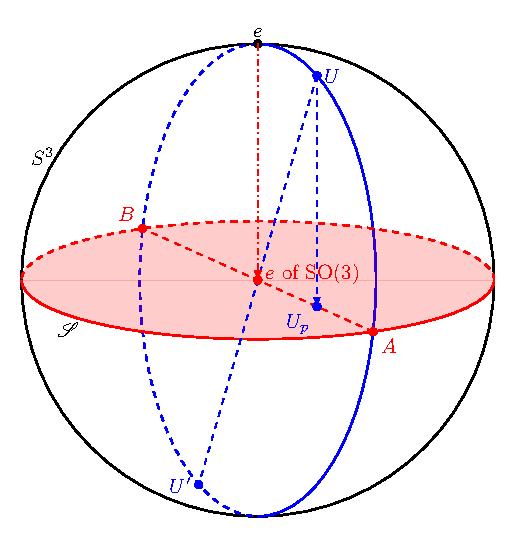
\includegraphics{../tikzpicture/SU2.pdf}
     \caption{SU(2)的流形}
     \label{SU(2)的流形图}
 \end{figure}
 我们压缩一个维度,用图直观说明一下,如图\ref{SU(2)的流形图}所示,我们以三维球面$S^3$代表SU(2)的流形,恒等元在北极点,用一个平面切出的圆环实际上是一个三维球壳;接下来我们直观的说明$\pi:SU(2)\rightarrow SO(3)$是一个2对1的一个映射;
 首先我们把目光聚焦在赤道面上也就是红色面,其中SU(2)在这里的应该是最外面的红线$\mathscr{S}$,加上内部的阴影和A、B的对径认同,则整个赤道面可以看作是SO(3)的流形,这一点不难想到,我们看恒等元e投影到赤道面上依旧是恒等元,同理北半球面如图
 所示与赤道面一一对应,而且是连续的映射,正逆皆如此,结果就是北半球面加上赤道线与赤道面同胚,就是流形之间的同胚.则与U对应的点$U_p$满足$U_p \in SO(3)$,图中U和U'是对径的两点,定义映射$$\pi:SU(2) \mapsto SO(3)\text{满足} \pi(U') = \pi(U) = U_p$$
 我们说SU(2)和SO(3)满足二对一的映射,$U_p$是两者一一对应的那个点.

 我们先说明SO(3)的非单连通性,考虑对径直线,由于对径认同,可以认为这是闭合的,但是不能通过连续变形为一点,所以不是单连通流形,就就像图中的$B\rightarrow e \rightarrow A$.
 \begin{definition}{同伦homotopic}{同伦}
     设M为连通流形,M中两条连续闭合曲线$C_1,C_2$称为彼此\textbf{同伦(homotopic)}的,若$C_1$可以连续变形为$C_2$.
 \end{definition}
 M中所有连续的闭曲线可以分为若干同伦类.单连通流形只有一个同伦类.

最后,我们定量给出映射$\pi:SU(2)\rightarrow SO(3)$并证明2对1的同态性.
前面我们给出了$\mathscr{SU}(2)$的基底$\{E_i = -i\tau_i/2\}$可对每一$\vec{v}\equiv (v^1,v^2,v^3) \in \mathbb{R}^3$构造一个$$\vec{v}\cdot \vec{E} = v^iE_i \in \mathscr{SU}(2)$$
\begin{note}
这里有一个问题,可以拓宽一下想法,就是前文的矩阵说$2\times 2$矩阵,而$v^i$理论上应该是$3\times 1$的列向量,带给我的第一感觉是存在问题,不满足矩阵乘法,实际上这里$v^i \in \mathbb{R}$
上面的意思是数乘.
\end{note}
给一个$U\in SU(2)$,令$A \equiv U(\vec{v}\vec{E})U^{-1}$,则
$$A^\dagger = \overline{(U(\vec{v}\vec{E})U^{-1})^T} = U(\overline{v\vec{v}\vec{E}^T})U^{-1} =  U(-\vec{v}\vec{E})U^{-1} = -A$$
最后一步要对每一个基矢验证,结果就是需要提出一个负号,其次我们来求迹,首先给出一个引理
\begin{lemma}
    $$tr(AB) = tr(BA),\quad A,B\text{都是矩阵}$$
\end{lemma}
proof:其实证明不难,用指标就可以看出是相同的数求和
$$tr(AB) = tr(A_{ij}B^{jk}) = A_{ij}B^{ji} = B^{ji}A_{ij} = tr(B^{ki}A_{ij}) = tr{BA}$$
然后我们来求迹
$$tr(A) = tr(U(\vec{v}\vec{E})U^{-1}) = tr(\vec{v}\vec{E}U^{-1}U) = tr(\vec{v}\vec{E}) = 0$$
最后一步是由基矢的特点给出的.所以$A \in \mathscr{SU}(2)$

这样便存在唯一的$v'^i \in \mathbb{R},\quad i = 1,2,3 $满足
$$U(\vec{v}\vec{E})U^{-1} = \vec{v'}\cdots \vec{E}$$
表明U诱导出一个映射$Z:\mathbb{R}^3 \rightarrow \mathbb{R}^3$满足$Z(\vec{v}) \equiv \vec{v}'$

先来证明一个有用的等式$\det(\vec{v}\cdot \vec{E}) = \frac{|\vec{v}|^2}{4}$
$$\det{\vec{v}\cdot \vec{E}} = \det{v^i E_i} = \det{v^i E_i} = \det \begin{bmatrix}
    -\frac{i}{2}(v_3)&-\frac{i}{2}(v_1 - iv_2)\\
    -\frac{i}{2}(v_1 + iv_2)&-\frac{i}{2}(-v_3)\\
\end{bmatrix} = \frac{(v^1)^2 + (v_2)^2 +v_3^2}{4} = \frac{v^2}{4}$$
所以有$$|v'|^2 = 4 \det(\vec{v}' \cdot \vec{E}) = 4\det{U(\vec{v}\vec{E})U^{-1}}=4 \det U \det (\vec{v}\vec{E})\det U^{-1} = |v|^2 $$
也就是说映射$Z:\mathbb{R}^3 \rightarrow \mathbb{R}^3$就是一个保长的一个映射,所以$Z\in O(3)$

如果$\det{Z} > 0$那么它就是SO(3)的群元.这里先说明一下,行列式的定义我们给出过详见\ref{def:行列式},本质上是一个变换系数,如果是负的话,会把右手系变成左手系;正的话则相反.
先来看一个等式
\begin{equation*}
[\vec{u} \cdot \vec{E}, \vec{v} \cdot \vec{E}]=u^{i} v^{j}\left[E_{i}, E_{j}\right]=u^{i} v^{j} \varepsilon_{i j}^{k} E_{k}=(\vec{u} \times \vec{v})^{k} E_{k}=(\vec{u} \times \vec{v}) \cdot \vec{E},\\
\end{equation*}
故
\begin{align*}
	Z(\vec{u} \times \vec{v}) \cdot \vec{E}=U & {[(\vec{u} \times \vec{v}) \cdot \vec{E}] U^{-1}=U[\vec{u} \cdot \vec{E}, \vec{v} \cdot \vec{E}] U^{-1}=\left[U(\vec{u} \cdot \vec{E}) U^{-1}, U(\vec{v} \cdot \vec{E}) U^{-1}\right] } \\
	                                          & =[(Z \vec{u}) \cdot \vec{E},(Z \vec{v}) \cdot \vec{E}]=[(Z \vec{u}) \times(Z \vec{v})] \cdot \vec{E},
\end{align*}
这里是正的变换,即$\det Z >0$;给出结论,存在映射$\pi : SU(2) \rightarrow SO(3)$满足$\pi(U) = Z$

我们从直观的看,是一个2对1的一个映射,而且$U' = -U$整理一下思路,就是要证明$\forall U,U' \in SU(2)$有$$\pi(U') = \pi(U)\Leftrightarrow U' = \pm U$$
令$Z \equiv \pi(U),Z' \equiv \pi(U')$
则有$$(Z \vec{v}) \cdot \vec{E}=U(\vec{v} \cdot \vec{E}) U^{-1}, \quad\left(Z^{\prime} \vec{v}\right) \cdot \vec{E}=U^{\prime}(\vec{v} \cdot \vec{E}) U^{\prime-1}, \quad \forall \vec{v} \in \mathbb{R}^{3} $$
若$  U^{\prime}= \pm U $, 则上式导致$$\left(Z^{\prime} \vec{v}\right) \cdot \vec{E}=( \pm U)(\vec{v} \cdot \vec{E})\left( \pm U^{-1}\right)=U(\vec{v} \cdot \vec{E}) U^{-1}=(Z \vec{v}) \cdot \vec{E}$$
故 $ Z^{\prime} \vec{v}=Z \vec{v}, \forall \vec{v} \in \mathbb{R}^{3}$ , 因而$  Z^{\prime}=Z $, 即$  \pi\left(U^{\prime}\right)=\pi(U) $. 反之, 若$  \pi\left(U^{\prime}\right)=\pi(U) $,
则有$  U^{\prime}(\vec{v} \cdot \vec{E}) U^{\prime-1}=U(\vec{v} \cdot \vec{E}) U^{-1} $, 所以$$U^{-1} U^{\prime}(\vec{v} \cdot \vec{E})=(\vec{v} \cdot \vec{E}) U^{-1} U^{\prime}, \quad \forall \vec{v} \in \mathbb{R}^{3}$$
作为$  2 \times 2  $复矩阵, $ U^{-1} U^{\prime} $ 总可表为$  I, E_{1}, E_{2}, E_{3} $ 的(实的)线性组合, 即$  \exists \alpha^{0}, \alpha^{i} \in \mathbb{R} $$  U^{-1} U^{\prime}=\alpha^{0} I+\alpha^{i} E_{i} $. 取$  \vec{v}  $
	使$  \vec{v} \cdot \vec{E}=E_{1} $, 代入上式后不难得到$  \alpha^{2}=\alpha^{3}=0 $(由李括号可知这两个左右交换的积不同,只能限定系数是0),同法可证$  \alpha^{3}=\alpha^{1}=0 $, 故$  U^{-1} U^{\prime}=\alpha^{0} I $,

	因而$  \alpha^{0}=\operatorname{det}\left(U^{-1} U^{\prime}\right),\left|\alpha^{0}\right|=1, \alpha^{0}= \pm 1 $. 于是$$  U^{-1} U^{\prime}= \pm I, U^{\prime}= \pm U $$
最后证明$  \pi  $为同态映射.
改写式子为$[\pi(U) \vec{v}] \cdot \vec{E}=U(\vec{v} \cdot \vec{E}) U^{-1}$,则$  \forall U^{\prime} \in \mathrm{SU}(2)  $有
$$\begin{array}{c}{\left[\pi\left(U^{\prime}\right) \pi(U) \vec{v}\right] \cdot \vec{E}=U^{\prime}[(\pi(U) \vec{v}) \cdot \vec{E}] U^{\prime-1}=U^{\prime}\left[U(\vec{v} \cdot \vec{E}) U^{-1}\right] U^{\prime-1}} \\=\left(U^{\prime} U\right)(\vec{v} \cdot \vec{E})\left(U^{\prime} U\right)^{-1}=\left[\pi\left(U^{\prime} U\right) \vec{v}\right] \cdot \vec{E},\end{array}$$
故$\pi(U')\pi(U) = \pi (U'U)\quad \forall U',U \in SU(2)$,所以$\pi : SU(2)\rightarrow SO(3)$是同态,保护的群乘法是李群乘法,所以是李群同态.
\chapter{李变换群和killing矢量场}
把流形$M$上的单参微分同胚群$\phi :\mathbb{R}\times M \rightarrow M$中的
\begin{definition}
	设G是李群,M是流形.$C^\infty$映射$\sigma:G\times M \rightarrow M$称为M上的一个\textbf{李变换群(Lie group of transformation)},若
	\begin{enumerate}
		\item $\forall g \in G, \sigma_g:M\rightarrow M $是微分同胚;
		\item $\sigma_{gh} = \sigma_g \circ \sigma_h, \forall g,h \in G$
	\end{enumerate}
\end{definition}
以复合映射定义群乘法,容易验证满足群乘法;恒等元是$\sigma_e$;还有就是$(\sigma_g)^{-1} = \sigma_{-g},\forall g \in G$.
同时还会有以下等式$$\sigma_p(g) = \sigma(g,p) = \sigma_g(p)\quad \forall g\in G, p \in M$$
李群按定义是一个高度抽象的概念,而李变换群就比较具体了,它的群元$\sigma_g$是流形M上的点变换(微分同胚),例如抽象的SO(3)可以借用一个2维球面$S^2$想象变得具体.
\begin{definition}
	从李群$G =\{g\}$到李变换群$\{\sigma_g: M\rightarrow M|g\in G\}$的同态映射$G \rightarrow \{\sigma_g\} $称为G的一个实现\textbf{实现{realization}},M称为\textbf{实现空间}.若此同态为同构,则称为
	\textbf{忠实(faith)表现}
\end{definition}
\begin{note}
	左不变映射$L_g$根据上面定义可以看作是忠实实现.
\end{note}
\begin{definition}
	李群G在流形M上的一个实现$G \rightarrow \{\sigma_g\}$称为G的一个\textbf{表示(representation)},若M是矢量空间且$\sigma_g : M\rightarrow M(\forall g \in G)$是线性变换.这时称为M为\textbf{表示空间}.同时把$\{\sigma_g\}$称为G的表示.
	若忠实实现是表示,则称为\textbf{忠实表示}.
\end{definition}

设$\gamma:\mathbb{R}\longrightarrow G$是G的、的与$A\in V_e$对应的单参子群,则$\gamma(t)$是G上的曲线.把群$\{\sigma_g \in |g\in G\}$中G的取值范围限制在$\gamma(t)$上,便得到子集$\{\sigma_{\gamma(t)}|t\in \mathbb{R}\}$,其中每个$\sigma_{\gamma(t)}: M\rightarrow M$
都是微分同胚,而且满足\[
	\sigma_{\gamma(t)}\circ \sigma_{\gamma(s)} = \sigma_{\gamma(t)\gamma(s)} = \sigma_{\gamma(t+s)}
\]可见G的每一个单参子群决定M上的一个单参微分同胚群.我们想找出与之对应的$C^\infty$矢量场$\bar{\xi}$.

因为$\bar{\xi}$的积分曲线与单参微分同胚群$\{\sigma_{\gamma(t)}| t \in \mathbb{R}\}$的轨道重合,所以可以得到在p点的切矢为
$\bar{\xi}_p,\quad \forall p \in M$.群$\{\sigma_{\gamma(t)}|t \in \mathbb{R}\}$ 过p点的集合是$\{\sigma_{\gamma_t}(p)|t\in \mathbb{R}\}$
则有\[
	\sigma_{\gamma(t)}(p) = \sigma(\gamma(t),p) = \sigma_p(\gamma(t))
\]于是有\[
	\bar{\xi}_p = \left.\dfrac{d}{dt}\right|_{t = 0} \sigma_p(\gamma(t)) = \sigma_{p*}\left.\dfrac{d}{dt}\right|_{t = 0} \gamma(t) = \sigma_{p*}A
\]
可见,给定李变换群$\sigma: G\times M\rightarrow M $,G的李代数$V_e$的每一个元素A会对应于M上的光滑矢量场(即$C^\infty$矢量场),也就是说存在映射$\chi:V_e \rightarrow \{\bar{\xi}\}$.

我们先来看一类特殊情况:M是带度规$g_{ab}$的流形,G是$(M,g_{ab})$的等度规群,李变换群$\sigma$的每一群元$\sigma_g : M\rightarrow M $
都是等度规映射.这时G的每一个单参子群$\gamma(t)$产生的单参微分微分同胚群$\{\sigma_{\gamma(t)}|t\in \mathbb{R}\}$会强化为单参等度规群,其轨道
切矢上的$\bar{\xi}$就是$(M,g_{ab})$的killing矢量场,引入$\mathscr{K}$代表M上的全部Killing
矢量场,则结论就是$$
	\{\bar{\xi}\} \subset \mathscr{K}$$
故$\chi$可以看作映射$V_e \rightarrow \mathscr{K}$上的线性映射.
\begin{lemma}
	Killing矢量场的对易子依旧是killing的.
\end{lemma}
proof:见第4章习题13.

那么我们完全可以以对易子作为李括号,则$\mathscr{K}$有李代数且有定理.\begin{theorem}
	映射$\chi:V_e \rightarrow \mathscr{K}$保李括号的程度满足式子$$
		\chi([A,B]) = -[\chi(A),\chi(B)]\quad \forall A,B \in V_e$$
\end{theorem}
这里书上没有证明,当结论记住吧.
定义映射$\psi (A) = - \chi(A)$,则$\psi$保李括号,即$$
	\psi([A,B]) = [\psi(A),\psi(B)],\quad \forall A,B \in V_e $$
那么$\psi$被称为李代数同态,因为每个完备的killing矢量场都能产生一个单参等度规群,故二者同维,则$\psi $是同构,而不完备的矢量场由于总有取值取不到,也就限制住李群只有恒等元,为0维.
\begin{theorem}
	$(M,g_{ab})$ 的等度规群的李代数$V_e$同构于其上的全体killing场的集合$\mathscr{K}$的李子代数;当每一killing场都完备时$V_e = \mathscr{K}$
	(李代数同构)
\end{theorem}
有了上面定理,我们可以借用killing矢量场的来计算群的结构常数,我们来看几个例子.
\begin{example}
	3维欧式空间$(\mathbb{R}^3,\delta_{ab})$中的二维球面$(S^2,h_{ab})$
\end{example}
这里我们要计算群的结构常数,给定的二维球面是$S^2 $是是一个给定度规的流形,对其进行变换的有意义的变换应该是要求保度规的,也就是O群,$S^2 $是嵌入到三维空间的二维流形,借用坐标表示
也就是存在3个参数所以是O(3)群,我们讨论的是killing矢量场,如果要求存在矢量变换要有连通性,对于包含恒等元的最适合的便是
SO(3)群.SO(3)的维度这样计算$$
	dim SO(3) = \frac{m(m-1)}{2}=\frac{3(3-1)}{2}= 3$$
也就是说SO(3)的变换会给出3个独立的killing矢量场.

这里我们还是给出如何求一个流形的killing矢量场,根据定理4-3-1,详见P109.给出killing矢量场满足矢量方程.
$$
	\nabla_{(a}\xi_{b)} = 0
$$
首先我们需要给出$S^2 $的度规,以及与其适配的导数算符.我们知道二维球面的线元满足$$
	ds^2 = d^2\theta + \sin^2\theta d^2\varphi
$$这里$\theta$为与z轴夹角,$\varphi $为与x轴夹角.
所以与之适配的度规便给出了来,这里以矩阵的形式表示为$$
	g_{\mu\nu} = \begin{bmatrix}
		1 & 0             \\
		0 & \sin^2 \theta
	\end{bmatrix}$$
不难给出$$
	g^{\mu\nu} = \begin{bmatrix}
		1 & 0                \\
		0 & \sin^{-2} \theta
	\end{bmatrix}$$
还需要计算克氏符,因为这里不是欧式空间,克氏符的计算公式如下所示$$
	\Gamma^{\sigma}{}_{\mu\nu} = \frac{1}{2}g^{\sigma \rho}(g_{\rho\mu,\nu} + g_{\nu\rho,\mu} - g_{\mu\nu,\rho})$$
这里$g_{ab,c}$表示$\partial_{c}g_{ab}$.把度规代入可以得到不同的分量,这里只计算一个,剩余直接给出结果.
\begin{align*}
	\Gamma^{1}{}_{22} & = \frac{1}{2} g^{1\rho}(\partial_{2}g_{\rho 2} + \partial_{2}g_{2 \rho} - \partial_{\rho}g_{22}) \\
	                  & = \frac{1}{2} (\partial_{2}g_{1 2} + \partial_{2}g_{21 } - \partial_{1}g_{22})                   \\
	                  & =- \frac{1}{2} \partial_{\theta} \sin^2\theta                                                    \\
	                  & =-\sin \theta \cos \theta
\end{align*}
我们给出所有结果
\begin{align*}
	\Gamma^{1}{}_{11} & =0                        \\
	\Gamma^{1}{}_{12} & =0                        \\
	\Gamma^{1}{}_{21} & =0                        \\
	\Gamma^{1}{}_{22} & =-\sin \theta \cos \theta \\
	\Gamma^{2}{}_{11} & =0                        \\
	\Gamma^{2}{}_{12} & =\cot \theta              \\
	\Gamma^{2}{}_{21} & =\cot \theta              \\
	\Gamma^{2}{}_{22} & =0                        \\
\end{align*}
我们知道$$
	\nabla_a \xi_b = \partial_a \xi_b - \Gamma^{c}{}_{ab}\xi_c
$$
这里应该给出3个方程
\begin{align*}
	\nabla_{(1}\xi_{1)} & = 0 \Rightarrow \partial_{(1}\xi_{1)} - \Gamma^{c}{}_{11}\xi_c = 0  \\
	\nabla_{(1}\xi_{2)} & = 0 \Rightarrow  \partial_{(1}\xi_{2)} - \Gamma^{c}{}_{12}\xi_c = 0 \\
	\nabla_{(2}\xi_{2)} & = 0 \Rightarrow  \partial_{(2}\xi_{2)} - \Gamma^{c}{}_{22}\xi_c = 0 \\
\end{align*}
最后给出方程组
\begin{align*}
	 & \partial_{(1}\xi_{1)} = 0                                 \\
	 & \partial_{(1}\xi_{2)} - \cot \theta \xi_2 = 0             \\
	 & \partial_{(2}\xi_{2)} + \sin \theta \cos \theta \xi_1 = 0 \\
\end{align*}
接下来我们计算求解
\begin{align}
	 & \partial_{1}\xi_{1} = 0                                          \\
	 & \partial_{1}\xi_{2}+ \partial_{2}\xi_{1}-2 \cot \theta \xi_2 = 0 \\
	 & \partial_{2}\xi_{2} + \sin \theta \cos \theta \xi_1 = 0
\end{align}
2式对$\varphi$求偏导,同时把1和3式代入得到
$$
	\frac{\partial^2}{\partial^2 \varphi} \xi_1 + \xi_1 = 0
$$
可以得到$$
	\xi_1 = A\cos \varphi + B \sin \varphi$$
把上式代入式3,可得$$
	\xi_2 = -A \sin \theta \cos \theta \sin \varphi + B \sin \theta \cos \theta \cos \varphi + C(\theta)$$
再度代回式2,可以得到$$
	\frac{\partial C(\theta)}{\partial \theta} - 2\cot \theta C(\theta) = 0$$
结果是$$
	C(\theta) = C \sin^2 \theta$$
\begin{note}
	如果有不会解得微分方程,可以借助mathmatical等工具求解,这里是使用的是分量变量法解得的.
\end{note}
到目前为止,汇总结果\begin{align*}
	\xi_1 & = A\cos \varphi + B \sin \varphi                                                                    \\
	\xi_2 & =- A \sin \theta \cos \theta \sin \varphi + B \sin \theta \cos \theta \cos \varphi + C\sin^2 \theta
\end{align*}
\begin{note}
	这里需要着重说明一下上面两个式子的意义,首先$\xi_a$是二维球面的矢量场,取值为1,2是我们在选定好坐标系后给出的沿坐标的分量,也就是说
	上面这两个式子就是二维球面在球坐标系下的$\theta ,\varphi$两个方向的分量,而我们前面知道存在3个独立的killing矢量场,
	我们只需要凑出3个矢量作为基矢即可.
\end{note}
不妨令$A,B,C$轮流取1,其余取0给出3个对偶矢量来.然后使用度规给出矢量场
\begin{align*}
	 & A = 1,B=C=0 \rightarrow \xi^1 = g^{11}\xi_1 = \cos\varphi ,\quad \xi^2 =g^{22}\xi_2 = -\sin^{-2}\theta \sin\theta \cos\theta \sin\varphi = -\cot\theta\sin\varphi \\
	 & B = 1,A=C=0 \rightarrow \xi^1 = g^{11}\xi_1 = \sin\varphi ,\quad \xi^2 =g^{22}\xi_2 =\sin^{-2}\theta \sin\theta \cos\theta \cos\varphi =\cot\theta\cos\varphi     \\
	 & C = 1,B=A=0 \rightarrow \xi^1 = g^{11}\xi_1 =0 ,\quad \xi^2 =g^{22}\xi_2 = \sin^{-2}\theta \sin^2\theta  =1
\end{align*}
汇总给出的3个矢量场\begin{align}
	(\xi^a)_1 & = \sin \varphi \frac{\partial}{\partial \theta} +\cot \theta \cos \varphi\frac{\partial}{\partial \varphi} \\
	(\xi^a)_2 & = \cos \varphi \frac{\partial}{\partial \theta} -\cot \theta \sin \varphi\frac{\partial}{\partial \varphi} \\
	(\xi^a)_3 & = \frac{\partial}{\partial \varphi}
\end{align}
不难验证\begin{align*}
	[(\xi^a)_1,(\xi^a)_2] & =(\xi^a)_3 \\
	[(\xi^a)_2,(\xi^a)_3] & =(\xi^a)_1 \\
	[(\xi^a)_3,(\xi^a)_1] & =(\xi^a)_2 \\
\end{align*}
这可以看作李代数$\mathscr{SO}(3)$的结构常数表达式.
实际上,上面3个矢量场便是绕坐标轴旋转给出的矢量场,为了很好的说明其直观性,我们这里从几何的角度给出矢量场.

设球面上的点 \((x, y, z)\) 用球坐标表示为:
\[
	\begin{aligned}
		x & =  \sin\theta \cos\varphi, \\
		y & =  \sin\theta \sin\varphi, \\
		z & =  \cos\theta,
	\end{aligned}
\]
其中\(\theta \in [0, \pi]\) 是极角,\(\varphi \in [0, 2\pi)\) 是方位角.
当球面绕 \(x\)、\(y\)、\(z\) 轴微小旋转时,诱导出的矢量场分别为:

绕 \(x\) 轴旋转一个小角度 \(\delta\alpha\),旋转矩阵为:
\[
	R_x(\delta\alpha) \approx \begin{bmatrix}
		1 & 0            & 0             \\
		0 & 1            & -\delta\alpha \\
		0 & \delta\alpha & 1
	\end{bmatrix}.
\]
因此点 \((x, y, z)\) 的变化为:
\[
	\delta\bm{r}_x = \begin{bmatrix}
		0  \\
		-z \\
		y
	\end{bmatrix} \delta\alpha.
\]
对应的诱导矢量场为:
\[
	\bm{v}_x = \begin{bmatrix}
		0  \\
		-z \\
		y
	\end{bmatrix}.
\]
绕 \(y\) 轴旋转一个小角度 \(\delta\beta\),旋转矩阵为:
\[
	R_y(\delta\beta) \approx \begin{bmatrix}
		1            & 0 & \delta\beta \\
		0            & 1 & 0           \\
		-\delta\beta & 0 & 1
	\end{bmatrix}.
\]
因此点 \((x, y, z)\) 的变化为:
\[
	\delta\bm{r}_y = \begin{bmatrix}
		z \\
		0 \\
		-x
	\end{bmatrix} \delta\beta.
\]
对应的诱导矢量场为:
\[
	\bm{v}_y = \begin{bmatrix}
		z \\
		0 \\
		-x
	\end{bmatrix}.
\]
绕 \(z\) 轴旋转一个小角度 \(\delta\gamma\),旋转矩阵为:
\[
	R_z(\delta\gamma) \approx \begin{bmatrix}
		1            & -\delta\gamma & 0 \\
		\delta\gamma & 1             & 0 \\
		0            & 0             & 1
	\end{bmatrix}.
\]
因此点 \((x, y, z)\) 的变化为:
\[
	\delta\bm{r}_z = \begin{bmatrix}
		-y \\
		x  \\
		0
	\end{bmatrix} \delta\gamma.
\]
对应的诱导矢量场为:
\[
	\bm{v}_z = \begin{bmatrix}
		-y \\
		x  \\
		0
	\end{bmatrix}.
\]
绕 \(x\)、\(y\)、\(z\) 轴的诱导矢量场在笛卡尔坐标系下分别为:
\[
	\bm{v}_x = \begin{bmatrix}
		0  \\
		-z \\
		y
	\end{bmatrix}, \quad
	\bm{v}_y = \begin{bmatrix}
		z \\
		0 \\
		-x
	\end{bmatrix}, \quad
	\bm{v}_z = \begin{bmatrix}
		-y \\
		x  \\
		0
	\end{bmatrix}.
\]
这些矢量场表示了球面上的每一点在对应轴的微小旋转下的速度方向和大小.这就是我们寻找的killing矢量场.换成$\theta,\varphi$
换成$\theta,\varphi$表示的坐标系我们有:
\begin{align*}
	\bm{v}_x & = -z \frac{\partial}{\partial y} + y \frac{\partial}{\partial z}=-\cos \theta \frac{\partial}{\partial y} + \sin\theta \sin\varphi \frac{\partial}{\partial z}               \\
	\bm{v}_y & =  z \frac{\partial}{\partial x} - x \frac{\partial}{\partial z}=\cos \theta \frac{\partial}{\partial x} -\sin \theta \cos \varphi  \frac{\partial}{\partial z}              \\
	\bm{v}_z & = -y \frac{\partial}{\partial x} + x \frac{\partial}{\partial y}=-\sin \theta \sin \varphi \frac{\partial}{\partial x} + \sin\theta \cos \varphi \frac{\partial}{\partial y}
\end{align*}
接下来我们转换基矢,这里我们更详细一些:
\begin{align*}
	\frac{\partial}{\partial x} & = \frac{\partial \theta}{\partial x}\frac{\partial}{\partial \theta}+\frac{\partial \varphi}{\partial x}\frac{\partial}{\partial \varphi}= \cos \theta \cos \varphi \frac{\partial}{\partial \theta}-\frac{\sin \varphi}{\sin \theta}\frac{\partial}{\partial \varphi} \\
	\frac{\partial}{\partial y} & = \frac{\partial \theta}{\partial y}\frac{\partial}{\partial \theta}+\frac{\partial \varphi}{\partial y}\frac{\partial}{\partial \varphi}= \cos \theta \sin \varphi\frac{\partial}{\partial \theta}+\frac{\cos \varphi}{\sin \theta}\frac{\partial}{\partial \varphi}  \\
	\frac{\partial}{\partial z} & = \frac{\partial \theta}{\partial z}\frac{\partial}{\partial \theta}+\frac{\partial \varphi}{\partial z}\frac{\partial}{\partial \varphi}=-\sin \theta \frac{\partial}{\partial \theta}                                                                                \\
\end{align*}
代入可以求得矢量场
\begin{align*}
	\bm{v}_x & =-\sin \varphi \frac{\partial}{\partial \theta} -\cot \theta \cos \varphi\frac{\partial}{\partial \varphi} \\
	\bm{v}_y & = \cos \varphi \frac{\partial}{\partial \theta} -\cot \theta \sin \varphi\frac{\partial}{\partial \varphi} \\
	\bm{v}_z & = \frac{\partial}{\partial \varphi}
\end{align*}可见在killing矢量空间.

本例结束后面还有几个例子,详见书P770
\chapter{伴随表示和killing型}
\section{伴随表示}
设V是m($<\infty$)维实矢量空间,令$$
	\mathscr{L}(V) \equiv \{\text{线性变换}\psi:V \rightarrow V\} \equiv \mathscr{T}_V(1,1)$$
则$\mathscr{L}(V)$是$m^2$维矢量空间,我们给其定义乘法$$
	\psi \varphi:= \psi\circ \varphi \quad\forall \psi,\varphi \in \mathscr{L}(V)$$然后我们就可以定义李括号为
$$
	[\psi,\varphi] := \psi \varphi - \varphi \psi$$
从而使得$\mathscr{L}(V)$成为$m^2$李代数.
\begin{definition}
	李代数同态映射$\beta : \mathscr{G}\rightarrow \mathscr{L}(V)$称为\textbf{李代数$\mathscr{G}$的表示}
\end{definition}
同一李群(李代数)可能有不同的表示,本节介绍李群和李代数的伴随表示,根据定义\ref{def:同构},对任意群G的群元可构造映射$$
	I_g:G\rightarrow G \Longrightarrow I_g(h) := ghg^{-1},\quad \forall h \in G $$称为自同构映射,对于李群而言,这还是个微分同胚,所以可以称为李群同构.根据定义
$I_g(e) = e$,所以这个映射在e点诱导的推前映射(切映射)是$V_e \rightarrow V_e$的映射,记为$\mathscr{A}\!d_g$,因为$V_e$就是G的李代数$\mathscr{G}$,故而
$\mathscr{A}\!d_g:\mathscr{G}\rightarrow \mathscr{G}$是线性变换.最后需要强调的一点,虽然$I_g$作用到$e$为$e$,但是不代表$\mathscr{A}\!d_g$会得到相同的切矢,所以对应的曲线不同.
\begin{theorem}
	设$\mathscr{G}$是李群G的李代数,则有$$
		\exp(t (\mathscr{A}\!d_g A)) = g(\exp tA)g^{-1}$$
\end{theorem}
proof: 设$\gamma(t) = \exp(tA),\gamma'(t) = g(\exp tA)g^{-1}$,首先$\gamma(t)$是单参子群,且方程左面是$\mathscr{A}\!d_g A$生成的,见定理\ref{thm:G-4-4},下面我们证明
$\gamma'(t)$也是单参子群.$$
	\gamma'(t+s) = g(\exp(t+s)A)g^{-1} = g(\exp(tA) \exp (sA))g^{-1} = g(\exp(tA)g^{-1}g\exp(sA)g^{-1} = \gamma'(t)\gamma'(s)$$
所以要想证明方程相等,只需要证明$\gamma'(t)$在恒等元的切矢为$\mathscr{A}\!d_g$,证明如下:$$
	\left.\frac{d}{dt}\right|_0 [g\exp(tA)g^{-1}] = \left.\frac{d}{dt}\right|_0 [I_g \exp(tA)] = I_{g*}\left.\frac{d}{dt}\right|_0 [\exp(tA)] = I_{g*}A = \mathscr{A}\!d_g A$$定理得证.
\begin{theorem}{}{G-8-2}
	设H是李群G的正规子群(定义见\ref{def:正规子群}),$\mathscr{H}$是H的李代数,则$$
		\mathscr{A}\!d_gB \in \mathscr{H},\quad \forall B \in \mathscr{H},g\in G$$
\end{theorem}
首先B是某个李代数,会生成一个单参子群$\exp(tB)$,又因为是正规子群所以$g\exp(tB)g^{-1}\subset H$,可见生成的单参子群也是H的单参子群,又因为$$
	\exp(t (\mathscr{A}\!d_g B)) = g(\exp tB)g^{-1}$$
可见$\mathscr{A}\!d_gB \in \mathscr{H}$
\begin{theorem}{}{G-8-3}
	设$\mathscr{G}$是李群G的李代数,则$\forall A,B \in \mathscr{G}$有$$
		[A,B] = \left.\frac{d}{dt}\right|_{t=0} (\mathscr{A}\!d_{(\exp tA)}B)$$
\end{theorem}
设$\phi$是由A产生的单参微分同胚群.
同定理\ref{thm:G-5-3}的证明$$
	[A,B] = [\bar{A},\bar{B}]_e = (\mathscr{L}_{\bar{A}}\bar{B})_e = \left.\frac{d}{dt}\right|_{t=0}(\phi_{-t*}\bar{B}_{\phi_{t}(e)})$$
因为定理\ref{thm:G-4-5},有$\phi_t(e) = e (\exp(tA)) = \exp(tA)$,则有$\bar{B}_{\phi_t(e)} = L_{\exp(tA)*}B$,则$$
	[A,B] = \left.\frac{d}{dt}\right|_{t=0}[(\phi_{-t} \circ L_{\exp(tA)})_{*}B]$$
另一方面有$$
	I_{\exp (tA)}(g) = \exp(tA) g \exp(-tA) = \phi_{-t}[\exp (tA)(g)] = \phi_{-t}[L_{\exp(tA)}(g) = (\phi_{-t}\circ L_{\exp(tA)}(g)$$
即$I_{\exp(tA)} = \phi_{-t}\circ L_{\exp (tA)}$,代入前面式子$$
	[A,B] = \left.\frac{d}{dt}\right|_{t=0}(I_{\exp(tA)*}B) = \left.\frac{d}{dt}\right|_{t=0}(\mathscr{A}\!d_{\exp(tA)}B)$$
\begin{theorem}
	设H是连通李群G的连通李子群,$\mathscr{H}$和$\mathscr{G}$分别是H和G的李代数,则H是G的正规子群$\Leftrightarrow$ $\mathscr{H}$是$\mathscr{G}$的理想(理想的定义见\ref{def:理想}).
\end{theorem}
\begin{proof}
	\begin{enumerate}
		\item ($\Rightarrow$) 由定理\ref{thm:G-8-2}知$\mathscr{A}\!d_{\exp(tA)}B \in \mathscr{H},\quad \forall A \in \mathscr{G} ,B\in \mathscr{H}, t \in \mathbb{R}$根据定理\ref{thm:G-8-3},$[A,B] \in \mathscr{H}$,根据理想的定义,$\mathscr{H}$是$\mathscr{G}$的理想.
		\item ($\Leftarrow$) \begin{lemma}
			      只要H是连通李群的连通李子群,则$\forall h \in H,\exists B_1,B_2,\cdots \in \mathscr{H}$使得$h = \exp(B_1)\exp(B_2)\cdots$(有限个指数之积)
		      \end{lemma}引理就交给数学家证明吧.

		      当$h = \exp(B),B\in \mathscr{H}$时$$
			      ghg^{-1} = g(\exp{B})g^{-1} = \exp(\mathscr{A}\!d_gB) \in H$$当$h = \exp(B_1) \exp(B_2) \cdots$则有$$
			      ghg^{-1} = g\exp(B_1) \exp(B_2)\cdots h^{-1} = g\exp(B_1) g^{-1}g\exp(B_2)\cdots h^{-1} = h_1 h_2 \cdots \in H$$则H是G的正规子群.
	\end{enumerate}
	\begin{note}
		理想在李代数的地位就是正规子群在群论的地位.
	\end{note}
\end{proof}
因为推前映射的线性性,不难知道$\mathscr{A}\!d_g:\mathscr{G}\xrightarrow{\text{线性}} \mathscr{G} \Rightarrow \mathscr{A}\!d_g\in \mathscr{L}(\mathscr{G})$,由此可见,每有一个g便可以通过映射$\mathscr{A}\!d:g\mapsto \mathscr{A}\!d_g$获得一个$\mathscr{L}(\mathscr{G})$的元素,
便有映射$$
	\mathscr{A}\!d:G\rightarrow \{\mathscr{G}\text{上可逆线性变换}\} \subset \mathscr{L}(\mathscr{G})$$

为什么会有可逆的?是因为$I_g:G\rightarrow G$是微分同胚,保证了$I_{g*}:\mathscr{G}\rightarrow \mathscr{G}$是同构映射
,便存在了逆映射.故{$\mathscr{G}$上可逆线性变换}对应于一个矩阵群$GL(m,\mathbb{R})$
\begin{theorem}
	$\mathscr{A}\!d:G \rightarrow \{\mathscr{G}\text{上的可逆线性变换}\}$是同态映射.
\end{theorem}
\begin{proof}
	$$\mathscr{A}\!d_{gh} = I_{gh*} =(I_{g}\circ I_{h})_* =I_{g*} \circ I_{h*}= \mathscr{A}\!d_g \circ \mathscr{A}\!d_h$$
	群元的复合映射就是群乘积,所以有$\mathscr{A}\!d_{gh} = \mathscr{A}\!d_g\cdot \mathscr{A}\!d_h$可见是同态映射.
\end{proof}
\begin{note}
	$I_{gh}(m) =ghmh^{-1}g^{-1} = I_{g}(I_h{m}) = I_{g}\circ I_{h} (m) \Rightarrow I_{gh} = I_g\circ I_h$
\end{note}
\begin{definition}
	同态映射$\mathscr{A}\!d:G \rightarrow \{\mathscr{G}\text{上可逆线性变换}\}$称为\textbf{李群G的伴随表示}(adjoint representation)
\end{definition}

定义映射$ad_A:=[A,B],\quad \forall B \in \mathscr{G}$由李括号的线性性可知$ad_A:\mathscr{G}\rightarrow \mathscr{G}$有如下两个性质:
\begin{enumerate}[label = (\alph*).]
	\item $\forall B_1,B_2\in \mathscr{G},\beta_1,\beta_2 \in \mathbb{R}$有$ad_A(\beta_1 B_1 +\beta_2B_2) = \beta_1 ad_A(B_1) + \beta_2 ad_A(B_2)$
	\item $\forall A_1,A_2\in \mathscr{G},\alpha_1,\alpha_2 \in \mathbb{R}$有$ad_{\alpha_1A_1 + \alpha_2 A_2}=\alpha_1 ad_{A_1} + \alpha_2 ad_{A_2}$
\end{enumerate}
性质(a)表明$ad_A$是$\mathscr{G}$上的线性变换,即$ad_A \in \mathscr{L}(\mathscr{G})$也可以看作(1,1)型张量,则有
$$
	(ad_A)^c{}_bB^b = [A,B]^c = C^c{}_{ab}A^aB^b,\quad \forall B^b \in \mathscr{G}$$
甩掉$B^b$后有$$
	(ad_A)^c{}_b = A^aC^c{}_{ab}
$$

映射$ad_A,\quad A \in \mathscr{G}$,虽然与$\mathscr{A}\!d_g,\quad g\in G$,但两者有如下关系:$$
	\mathscr{A}\!d_{exp(A)} = \text{Exp}(ad_A)$$
\begin{proof}
	构造映射$\gamma(t) = \mathscr{A}\!d_{\exp(tA)}$,$\gamma'(t) = \text{Exp}(t (ad_A))$,由定理\ref{thm:G-5-2},可见$\gamma'(t)$
	是由$ad_A$唯一决定的单参子群$\exp(t (ad_A))$,由于$\mathscr{A}\!d$是同态映射,再结合$\exp(t+s) A = \exp tA + \exp sA$说明
	$\gamma(t)$也是单参子群.又因为二者都是$\mathscr{G}\rightarrow \mathscr{G}$的映射,可见它们是同一个群.要证明二者相等,问题就比较简单了,只需要证明
	均过恒等元,且在切矢量相同即可,当$t = 0$时,两者不难看出是恒等元.我们来看切矢量,对于$\gamma(t)$由定理\ref{thm:G-8-3}可以看出$$
		\left.\frac{d}{dt}\right|_{t=0} (\mathscr{A}\!d_{\exp(tA)}) = ad_A $$
	对于$\gamma'(t)$,很明显,切矢为$ad_A$,所以可以得到结论$$
		\mathscr{A}\!d_{\exp(tA)} = \text{Exp}(t (ad_A))$$当$t = 1$
	时,便有我们想要的结果.

	\begin{note}以上证明为个人所想,如有错误请及时指出.\end{note}
\end{proof}

既然每一个$A \in \mathscr{G}$对应于一个$ad_A \in \mathscr{L}(\mathscr{G})$,便有从$\mathscr{G} \rightarrow \mathscr{L}(\mathscr{G})$
记作$ad : \mathscr{G}\rightarrow \mathscr{L}(\mathscr{G})$,性质(b)表明$ad$是线性映射,接下来我们来看映射是否是同态映射
李代数的同态映射,就是看它是否保李括号.
即\begin{align*}
	ad_{[A,B]}(C) & = [[A,B],C] = [A,[B,C]] + [B,[C,A]] \\
	              & = [A,[B,C]] -[B,[A,C]]              \\
	              & = ad_A(ad_B(C)) - ad_B(ad_A(C))     \\
	              & = (ad_A ad_B - ad_B ad_A)(C)
\end{align*}
由此可见$ad_{[A,B]} = [ad_A,ad_B]$
\begin{definition}
	同态映射$ad:\mathscr{G} \rightarrow \mathscr{L}(\mathscr{G}$ \textbf{李代数$\mathscr{G}$的伴随表示})
\end{definition}
五个映射总结\begin{enumerate}
	\item $I_g:G\rightarrow G$
	\item $\mathscr{A}\!d_g: \mathscr{G} \rightarrow \mathscr{G}$
	\item $\mathscr{A}\!d :G \rightarrow \{ \mathscr{G}\text{上可逆线性变换}\}$为李群的伴随表示
	\item $ad_A:\mathscr{G}\rightarrow \mathscr{G},\quad A\in \mathscr{G}$
	\item $ad : \mathscr{G} \xrightarrow{\text{线}} \mathscr{L}(\mathscr{G})$为李代数的伴随表示
\end{enumerate}
实际上$\mathscr{A}\!d_*$作为推前映射(切映射)与$ad$相等,有定理
\begin{theorem}
	映射$\mathscr{A}\!d_{*}: \mathscr{G} \rightarrow \mathscr{L}(\mathscr{G})$与$ad:\mathscr{G}\rightarrow \mathscr{L}(\mathscr{G})$相等
\end{theorem}
\begin{proof}
	只需要证明$(\mathscr{A}\!d_*A)(B) = ad_A(B)\quad \forall A,B \in \mathscr{G}$
	\begin{align*}
		\mathscr{A}\!d_* A = \mathscr{A}\!d_* [\left.\frac{d}{dt}\right|_{t=0}\exp(tA)] =   \left.\frac{d}{dt}\right|_{t=0}\mathscr{A}\!d(\exp (tA)) = \left.\frac{d}{dt}\right|_{t=0} \mathscr{A}\!d_{\exp(tA)}
	\end{align*}
	故有$$
		\mathscr{A}\!d_*A(B) = [\left.\frac{d}{dt}\right|_{t=0} \mathscr{A}\!d_{\exp(tA)}(B)] = \left.\frac{d}{dt}\right|_{t=0}(\mathscr{A}\!d_{\exp(tA}B) = [A,B] = ad_A(B)$$

\end{proof}
\section{killing型}
利用$\mathscr{G}$伴随表示可以定义映射$K:\mathscr{G}\times \\mathscr{G} \rightarrow \mathbb{R}$如下:
$$
	K(A,B):= \text{tr}(ad_A ad_B),\quad \forall A,B \in \mathscr{G}$$ 其中$ad_A,ad_B$是映射先后作用.加上求迹后,不难看出这是
一个对称的双线性映射,可以看作是$\mathscr{G}$上的$(0,2)$对称张量,在李代数理论中称为killing型.
\begin{theorem}
	$K([A,B],C) = K(A,[B,C]),\quad \forall A,B \in \mathscr{G}$
\end{theorem}
\begin{proof}
	\begin{align*}
		K([A,B],C) & = \text{tr}(ad_{[A,B]}ad_C)                  \\
		           & = \text{tr}([ad_A,ad_B]ad_C)                 \\
		           & = \text{tr}(ad_A ad_B ad_C - ad_B ad_A ad_C) \\
		           & = \text{tr}(ad_A ad_B ad_C - ad_A ad_C ad_B) \\
		           & = \text{tr}(ad_A[ad_B,ad_C])                 \\
		           & = K(A,[B,C])
	\end{align*}
	注意:求迹可以交换顺序,不影响结果.
\end{proof}

\end{document}
